\section{Model predictive control}\label{se:model_predictive_control}
In this section, the design of the controller is elaborated. First the control problem the design of the Model predictive controller (MPC). 

The simulation covered in chapter \ref{ch:simulation} is to be controlled with respect to the problems elaborated in section \ref{sec:problem_statement} and stated here. 
\begin{enumerate}
\item Flow variations due to large industries and natural phenomenons
\item Concentration variations due to large industries and natural phenomenons
\begin{enumerate}
	\item Chloride variations
	\item Phosphor variations
	\item Nitrogen variations
	\item Organic matter variations
\end{enumerate}
\end{enumerate}

From the problem statement, it is stated that flow and concentration variations must be kept to a minimum without causing any overflow in the sewer. To achieve this, tanks are used, these are placed in the sewer network to find locations where they are able to hold back disturbance that will otherwise cause flow and concentration variations into the WWTP. However, the output of these tanks must be controlled in a way where overflow in the tank is prohibited. Therefore the controller must control the output of these tanks in an optimal manner to keep the input variations to the WWTP at a minimum and still be controlled according to some constraints.

To obtain such an optimal behavior MPC is chosen as stated in section \ref{sec:problem_statement}. MPC solves a optimizations problem at each time instant, k, where the main point is to compute a control vector, u that is feed to the system. 

%is an advanced control method which depends on a dynamic model of the system. Where the model, constraints and a cost function is used to generate the most optimal sequence of control inputs to the system, thus obtaining a desired process behavior. However, only the first control input is used in the current timeslot. Hereafter, in the next timeslot, the MPC algorithm is recalculated to find the must optimal input signal for this timeslot and so on. In addition, MPC also take future disturbance into account thereby predicting an output sequence that is optimal including the disturbance. 
An MPC algorithm consists of:
\\ 
\textbf{Cost function} or control objective,$\CMcal{J}$, is an algorithm measuring e.g. the difference between future outputs and a reference while at the same time instant recognizing that any control action is costly for the system. Therefore the price is measured in the cost function over the prediction horizon, $H_p$. This function is therefore minimized with the respect to the future control vector to keep the cost minimized. Furthermore, only the first control input from the vector is used in each time instant thus this optimization is process is calculated at each time step where a new control input is calculated \cite{mpc_control_lecture_notes}.

\textbf{Constraints} is unique advantages of MPC. Constraints can be applied to the process variables e.g. constraints can be set on the states of the system not allowing them to go below a certain value or above. Constraints are usually written as inequality constraint $Ax\leq b$ where the constraint a subject to the optimization problem \cite{mpc_control_lecture_notes}.   

\textbf{Prediction model} for the MPC to be able to predict future system behavior it needs a model to predict from. The model describes the input output behavior of the system. The model will mainly be used to predict the output of the system over the prediction horizon \cite{mpc_control_lecture_notes}.  

% In figure \ref{fig:mpc_diagram} an illustration of a MPC controller is shown.
% \begin{figure}[H]
% 	\centering
% 	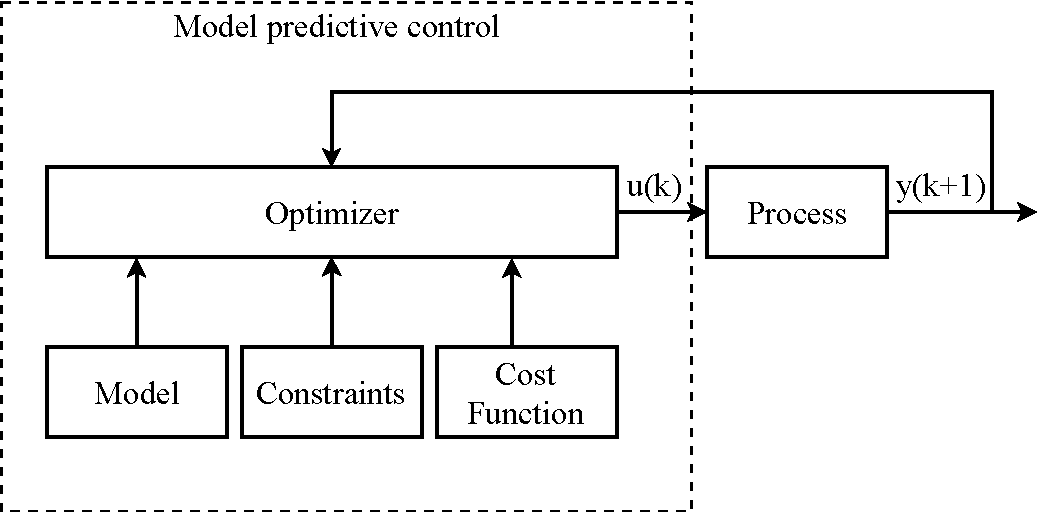
\includegraphics[width=0.60\textwidth]{report/control/pictures/mpc_diagram}
% 	\caption{Diagram of an MPC controller}
% 	\label{fig:mpc_diagram}
% \end{figure}



%The main advantage of MPC  Furthermore, MPC can be used with constraints to calculate the most optimal control output at the given timeslot and taking disturbance into the account. 
% In figure \ref{fig:control_of_sewer} it is shown that the MPC controller is setting the input to the pump.

% \begin{figure}[H]
% \centering
% 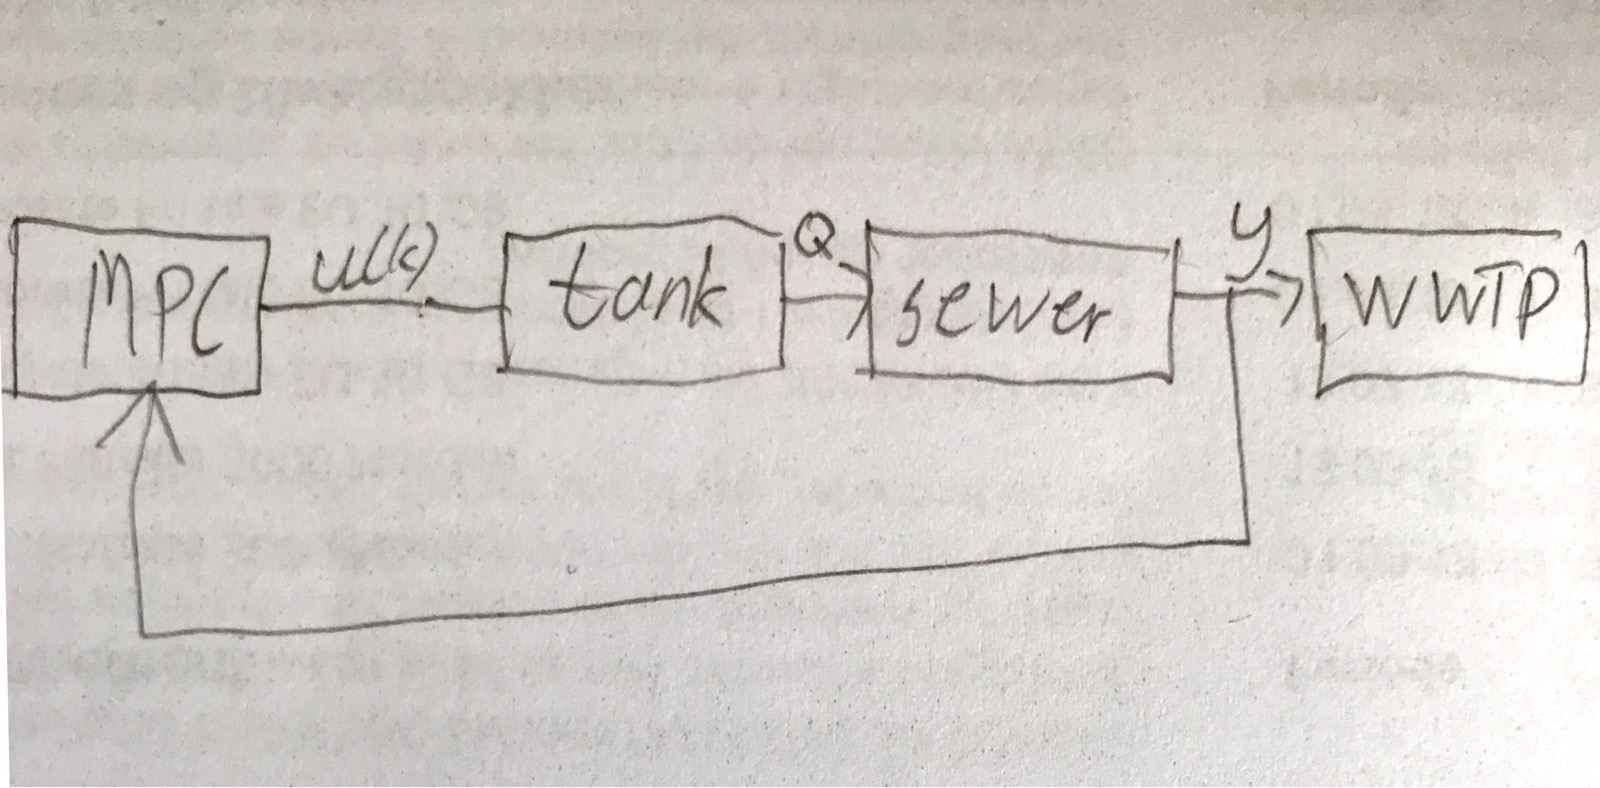
\includegraphics[width=0.8\textwidth]{report/control/pictures/control_of_sewer.jpg}
% \caption{Block diagram of the system.}
% \label{fig:control_of_sewer}
% \end{figure}\fxnote{Der skal staa pumpe i stedet for tank}

% Where the iteration the in the MPC block can be described with the following items. 
% \begin{enumerate}
%        	\item Measurement is taken on the output if possible or it is taken directly from the states. If a state measurement is not available the state is estimated.
%        	\item Calculates a optimal set of predicted values over the prediction horizon according to a cost function and the constraints.
%        	\item The first element of the calculated control sequence is used as the control input.
%        	\item Repeat from 1.
% \end{enumerate}       

For MPC to optimize the system a cost function must be written to penalize variations of the flow output $Q(k+i|k)$ and the concentration output $C(k+i|k)$. Where k defines the prediction time and i is a value going from 1 to $H_p$. The cost function for flow and concentration is:

\begin{equation}
\begin{aligned}
	 \CMcal{J} &= \sum_{i=1}^{H_p-1} || Q(k+i|k)C_1(k+i|k)-Q(k+i-1|k)C_1(k+i-1|k)||_{\CMcal{Q}(i)}^2 \\&+\sum_{i=1}^{H_p-1} || Q(k+i|k)C_2(k+i|k)-Q(k+i-1|k)C_2(k+i-1|k)||_{\CMcal{Q}(i)}^2 \\&+\sum_{i=1}^{H_p-1} || Q(k+i|k)C_3(k+i|k)-Q(k+i-1|k)C_3(k+i-1|k)||_{\CMcal{Q}(i)}^2\\&+\sum_{i=1}^{H_p-1} || Q(k+i|k)C_4(k+i|k)-Q(k+i-1|k)C_4(k+i-1|k)||_{\CMcal{Q}(i)}^2 \\& +\sum_{i=1}^{H_p-1} || Q(k+i|k)-Q(k+i-1|k)||_{\CMcal{Q}(i)}^2
\end{aligned}	
\end{equation}\fxnote{skal skrives så alle 4 koncentrationer er med, samt en for flow og et eller andet sted afgrænsning for liggetid i tank}
Where $\CMcal{J}$ is the cost function that needs to be minimized, Q is the flow, C is the concentration and $\CMcal{Q}$ is a weighting parameter. The concentrations $C_1, C_2, C_3$ and $C_4$ are respectively chloride, phosphor nitrogen and organic matter levels in the wastewater.However, It has been chosen to only look at flow variation in the simulation and thereby excluding concentrations from the cost function and retention time in the tank\fxnote{enten skal vi fra vaelge os den noget før eller os skal vi have fundet på en cost function til liggetid}. This has been done to limit the control problem and ease the computation, to begin with. Thereby the cost function has been rewritten to: 

\begin{equation}\label{eq:cost_function_height}
	 \CMcal{J} = \sum_{i=1}^{H_p-1} || \hat{y}(k+i|k)-\hat{y}(k+i-1|k)||_{\CMcal{Q}(i)}^2
\end{equation}
\begin{equation}
	\begin{aligned}
	\text{s.t.} \hspace{5mm}  \hat{x}(k+i+1) &= A\hat{x}(k+i|k)+B\hat{u}(k+i|k)+B_dd(k+i|k) \\
						      \hat{y}(k+i)&= C\hat{x}(k+i|k) \\
						     \underline{x} \leq \hat{x} \leq \overline{x}
	\end{aligned}
\end{equation}
Where Q has been replaced with the output y as it can be measured directly from the state space system. The hat denotes a small signal value and not an estimate for y. y corresponds to the height of the wastewater in the channel, however, it is the same to minimize height difference as the flow because both describe the variation in the output of the sewer. Furthermore, the cost function is subject to constraints for the states. The states have a lower and upper constraint corresponding respectively to the bottom of the channel and the top of the channel, denoted respectively with $\underline{x}$ and $\overline{x}$. In order for the controller to minimize the variations in the output, it must be able to predict future events from knowing the current state. Therefore, by iterating the linear model up to the prediction horizon the controller is able to predict future states \cite{maciejowski2002predictive}. The state equation is used for this predictive model: 

\begin{equation}
	\hat{x}(k+1|k) = A\hat{x}(k|k)+B\hat{u}(k|k) + B_dd(k|k)
\end{equation}

Where $\hat{u}(k|k)$ can be written as:

\begin{equation}
	\hat{u}(k) = \Delta \hat{u}(k|k)+u(k-1)
\end{equation}

Thus by using the state equation recursively the state equation can be predicted up to the prediction horizon as shown in equation \ref{eq:iterating_state_equation}: 

\begin{equation}\label{eq:iterating_state_equation}
\begin{aligned}
	\hat{x}(k+1|k) &= A\hat{x}(k|k)+B(\Delta \hat{u}(k|k)+u(k-1)) + B_dd(k|k)\\
	\hat{x}(k+2|k) &= A\hat{x}(k+1|k)+B\hat{u}(k+1|k)+ B_dd(k+1|k) \\
				   &= A^2\hat{x}(k|k)+AB(\Delta \hat{u}(k|k)+u(k-1))+AB_dd(k|k)\\ & + B\underbrace{(\Delta \hat{u}(k+1)+\Delta \hat{u}(k)+u(k-1))}_{\hat{u}(k+1|k)}+ B_dd(k+1|k) \\
				   &\hspace{2mm}\vdots\\
   \hat{x}(k+H_p|k)&= A^{H_p}\hat{x}(k|k)+(A^{H_p-1}+ \cdots +A +I)B\Delta\hat{u}(k|k)+\cdots\\
   				   &+ (A^{H_p-1}+ \cdots +A +I)B\Delta \hat{u}(k+H_p-1|k) \\	
   				   &+(A^{H_p-1}+ \cdots +A +I)Bu(k-1)\\
   				   &+A^{H_p-1}B_dd(k|k)  +\cdots+B_dd(k+H_p-1|k) 
\end{aligned}
\end{equation}\fxnote{skal lige gennemskue det her i morgen}
Here the first equation $\hat{x}(k+1|k)$ is inserted into the second and this is iterated up to the prediction horizon. This can be setup as prediction vectors and matrices denoted by $\CMcal{X,A,B,U,B}_d$ and $\CMcal{D}$:


% \begin{equation}\label{eq:iterating_state_equation}
% \begin{aligned}
% 	\hat{x}(k+1|k) &= A\hat{x}(k|k)+B\hat{u}(k|k) + B_dd(k|k)\\
% 	\hat{x}(k+2|k) &= A\hat{x}(k+1|k)+B\hat{u}(k+1|k)+ B_dd(k+1|k) \\
% 				   &= A^2\hat{x}(k|k)+AB\hat{u}(k|k)+AB_dd(k|k) + B\hat{u}(k+1|k) \\
% 				   &+ B_dd(k+1|k) \\
% 				   &\hspace{2mm}\vdots\\
%    \hat{x}(k+H_p|k)&= A\hat{x}(k+H_p-1|k)+B\hat{u}(k+H_p-1|k)+B_dd(k+H_p-1|k)\\
%    				   &= A^{H_p}\hat{x}(k|k)+A^{H_p-1}B\hat{u}(k|k)+A^{H_p-1}B_dd(k|k)+\cdots+\\
%    				   &+B\hat{u}(k+H_p-1|k)+B_dd(k+H_p-1|k)
% \end{aligned}
% \end{equation}


\begin{equation}\label{eq:lifted_state_equation}
\begin{aligned}
	  \underbrace{\begin{bmatrix}
	  \hat{x}(k+1|k) 	\\
	  \hat{x}(k+2|k) 	\\
	  \vdots 			\\
	  \hat{x}(k+H_p|k) 	\\
	   \end{bmatrix}}_{\CMcal{X}}
	 &=
	\underbrace{\begin{bmatrix}
		A \\
		A^2 \\
		\vdots \\
		A^{H_p} \\
	\end{bmatrix}}_{\CMcal{A}}
	\hat{x}(k|k) \\&+
	\underbrace{\begin{bmatrix}
		B 		 &0			 &\cdots	& 0		\\
		AB  	 &B  		 & \cdots& 0		\\
		\vdots 	 &\vdots	 & \ddots&\vdots	\\
		A^{H_p-1}B&A^{H_p-2}B&\cdots &B 
    \end{bmatrix}}_{\CMcal{B}}
    	\underbrace{\begin{bmatrix}
	\hat{u}(k|k)\\
	\hat{u}(k+1|k)\\
	\vdots\\
	\hat{u}(k+H_p-1|k)
	\end{bmatrix}}_{\CMcal{U}} \\ &+ 
    \underbrace{\begin{bmatrix}
    	B_d 	    &0	         &\cdots & 0		\\
		AB_d  	    &B_d  	     & \cdots& 0		\\
		\vdots 	    &\vdots	     & \ddots&\vdots	\\
		A^{H_p-1}B_d&A^{H_p-2}B_d&\cdots &B_d 
 %   	B & \cdots & 0 \\
 %    	AB+B & \cdots & 0 \\
 %    	\vdots & \ddots & \vdots \\
 %    	\sum_{i=0}^{H_u-1}A^i B & \cdots & B \\
 %    	\sum_{i=0}^{H_u}A^i B & \cdots & AB+B\\
 %    	\vdots & \vdots & \vdots \\
 %    	\sum_{i=0}^{H_p-1}A^i B & \cdots & \sum_{i=0}^{H_p-H_u}A^i B \\
	  \end{bmatrix}}_{\CMcal{B}_d} 
	\underbrace{\begin{bmatrix}
	\hat{d}(k|k)\\
	\hat{d}(k+1|k)\\
	\vdots\\
	\hat{d}(k+H_p-1|k)
	\end{bmatrix}}_{\CMcal{D}}
	\end{aligned}
\end{equation}

Where $\CMcal{X}$ is the predicted state vector for the entire prediction horizon. $\CMcal{A}$ is the state matrix up to the prediction horizon. $x(k|k)$ is the initial state and is used to predict the hole prediction horizon, $\CMcal{B}$ is the input matrix for the prediction horizon, $\CMcal{U}$ is the predicted input vector, which consists of all the predicted inputs from the current timestep until $(k+H_p-1)$. $\CMcal{B}_d$ is the disturbance matrix for the prediction horizon and $\CMcal{D}$ is the disturbance vector. 

This iteration process is also done for the output equation:

\begin{equation}\label{eq:lifted_output_equation}
	\CMcal{Y}(k)= 
	\underbrace{\begin{bmatrix}
	\hat{y}(k+1|k)\\
	\hat{y}(k+2|k)\\
	\vdots\\
	\hat{y}(k+H_p-1|k)
	\end{bmatrix}}_{\CMcal{Y}}
	= 
	\underbrace{\begin{bmatrix}
	C 		& 0 	&\cdots	& 0\\
	0 		& C 	&\cdots & 0 \\
	\vdots	& \vdots&\ddots & 0\\
	0 		& 0		&0 		& C
	\end{bmatrix}}_{\CMcal{C}}
	  \begin{bmatrix}
	  \hat{x}(k+1|k) 	\\
	  \hat{x}(k+2|k) 	\\
	  \vdots 			\\
	  \hat{x}(k+H_p|k) 	\\
	   \end{bmatrix}
\end{equation}
Where $\CMcal{C}$ is a diagonal matrix with the output matrix C and $\CMcal{X}$ the predicted state vector. By inserting the predicted state equation \ref{eq:lifted_state_equation}, into the predicted output equation \ref{eq:lifted_output_equation} the following is achieved:

% \begin{equation}\label{eq:output_eq_with_state_eq}
% 	\CMcal{Y}(k) =  \CMcal{C}\CMcal{A}x(k) +  \CMcal{C}\CMcal{B}\CMcal{U}(k) +\CMcal{C}\CMcal{B}_d\CMcal{D}(k)
% \end{equation}   
\begin{equation}\label{eq:output_eq_with_state_eq}
	\CMcal{Y}(k) =  \CMcal{C}\CMcal{A}x(k) +  \CMcal{C}\CMcal{B}u(k-1)+ \CMcal{C}\CMcal{B}_f\Delta \CMcal{U} +\CMcal{C}\CMcal{B}_d\CMcal{D}(k)
\end{equation}  

By using the following notation on equation \ref{eq:output_eq_with_state_eq}:


\begin{equation}
 \psi = \CMcal{C}\CMcal{A}  \hspace{5mm} \gamma = \CMcal{C}\CMcal{B} \hspace{5mm} \Omega = \CMcal{C}\CMcal{B}_f\Delta \CMcal{U}\hspace{5mm}  \Theta = \CMcal{C}\CMcal{B}_{d}
\end{equation}

The predicted output equation can be rewritten as: 

% \begin{equation}\label{eq:lifted_output_with_states_inserted}
% 	\CMcal{Y}(k) = \psi x(k) + \gamma \CMcal{U}(k) + \Theta \CMcal{D}(k)
% \end{equation}


\begin{equation}\label{eq:lifted_output_with_states_inserted}
	\CMcal{Y}(k) = \psi x(k) + \gamma u(k-1) +\Omega\Delta\CMcal{U}+ \Theta \CMcal{D}(k)
\end{equation}

To be able to use the cost function, equation \ref{eq:cost_function_height}, it has to be rewritten so the predicted output equation can be used. This is done by replacing the output y with the predicted output $\CMcal{Y}$ thereby the following is obtained:

\begin{equation}\label{eq:new_the_cost_function_yeah}
	\CMcal{J} = ||\CMcal{Y}(k)-\CMcal{Y}(k-1)||_{\CMcal{Q}(i)}^2
\end{equation}

%Where the difference between $\CMcal{Y}(k)$ and $\CMcal{Y}(k-1)$ can be expressed as:

% \begin{equation}
% 	\Delta \CMcal{Y}(k) =\CMcal{Y}(k)-\CMcal{Y}(k-1) 
% \end{equation}

% Thereby the following cost function is achieved:

% \begin{equation}\label{eq:delta_cost_function}
% 	J = \Delta\CMcal{Y}(k)^T \cdot Q \cdot \Delta\CMcal{Y}(k)
% \end{equation}

To be able to write the cost function as quadratic and linear terms of the predicted output $\Delta\CMcal{U}$, equation \ref{eq:lifted_output_with_states_inserted} is therefore inserted into equation \ref{eq:new_the_cost_function_yeah} and thereby the following is obtained:

% \begin{equation}\label{eq:cost_function_with_all_the_crap}
% 	\CMcal{J} = (\psi\Delta \hat{x}(k) + \gamma\Delta \CMcal{U}(k) + \Theta\Delta \CMcal{D}(k))^T\cdot Q \cdot (\psi\Delta \hat{x}(k) + \gamma\Delta \CMcal{U}(k) + \Theta\Delta \CMcal{D}(k))
% \end{equation}

\begin{equation}\label{eq:cost_function_with_all_the_crap}
\begin{aligned}
	\CMcal{J} 	&= (\psi \hat{x}(k) + \gamma u(k-1)+ \Omega \Delta \CMcal{U} + \Theta\CMcal{D}(k))^T\cdot Q \cdot (\psi \hat{x}(k) \\
				&+ \gamma u(k-1)+\Omega \Delta \CMcal{U} + \Theta\CMcal{D}(k))
\end{aligned}
\end{equation}

The term on the right hand side of equation \ref{eq:cost_function_with_all_the_crap} is equal to:

\begin{equation}\label{eq:cost_function_big_eq}
	\begin{aligned}
	&(\psi \hat{x}(k) + \gamma u(k-1)+\Omega\Delta\CMcal{U}(k) + \Theta\Delta \CMcal{D}(k))^T\cdot Q \cdot (\psi \hat{x}(k) + \gamma u(k-1)+\Omega\Delta\CMcal{U}(k) \\
	& + \Theta\Delta \CMcal{D}(k)) = \\
	&  \hat{x}(k)^T\psi ^T Q \psi  \hat{x}(k) +  \hat{x}(k)^T \psi ^T Q \gamma u(k-1)+ \underbrace{\hat{x}(k)^T \psi ^T Q \Omega\Delta\CMcal{U}(k)}_{Linear}\\
	& + \hat{x}(k)^T \psi ^T Q \Theta  \CMcal{D}(k) \\
	&+ u(k-1)^T \gamma ^T Q \psi \hat{x}(k) +  u(k-1)^T\gamma ^T Q \gamma u(k-1) +\underbrace{ u(k-1)^T \gamma Q \Omega\Delta\CMcal{U}(k)k)}_{Linear}\\
	&+ u(k-1)^T \gamma ^T Q\Theta \CMcal{D}(k) \\ 
	&+ \underbrace{\Delta\CMcal{U}(k)^T\gamma^TQ \psi  \hat{x}(k)}_{Linear} +  \underbrace{\Delta\CMcal{U}(k)^T\gamma^TQ \gamma u(k-1)}_{Linear}+ \underbrace{\Delta\CMcal{U}(k)^T\gamma^TQ \Omega\Delta\CMcal{U}(k)}_{Quadradic} \\
	&+ \underbrace{\Delta\CMcal{U}(k)^T\gamma^T Q \Theta  \CMcal{D}(k)}_{Linear} \\
	&+\CMcal{D}(k)^T \Theta ^T Q  \psi  \hat{x}(k)	+  \CMcal{D}(k)^T \Theta ^T Q \gamma u(k-1)+ \underbrace{\CMcal{D}(k)^T \Theta ^T Q   \Omega\Delta\CMcal{U}(k)}_{Linear}\\
	&+ \CMcal{D}(k)^T \Theta ^T Q \Theta \CMcal{D}(k)
	\end{aligned}
\end{equation}

Here the quadratic and linear terms of $\Delta \CMcal{U}$ are denoted respectively, the remaining terms are the constants and these are not denoted in the equation, however, they will be referred to in the following equations as, c. The quadratic variables are collected in: 

\begin{equation}\label{eq:quadratic_h_matrix}
	\CMcal{H} = \Omega^T Q\Omega 
\end{equation}

And the linear variables are collected in:
\begin{equation}
	\begin{aligned}
	\CMcal{G} &= 2 \cdot \hat{x}(k)^T\psi^T Q \Omega+2\cdot u(k-1)^T\gamma^T Q\Omega+2\cdot  \CMcal{D}(k)^T\Theta^T Q \Omega
	\end{aligned}
\end{equation}

Thereby inserting these expressions in equation \ref{eq:cost_function_big_eq} the final cost function is obtained:

\begin{equation}\label{eq:the_cost_function}
	\min_{\Delta \CMcal{U}(k)} \CMcal{J}(\Delta \CMcal{U}(k)) =\min_{\Delta \CMcal{U}(k)} \Delta \CMcal{U}(k)^T\CMcal{H}\Delta \CMcal{U}(k)+\CMcal{G}\Delta \CMcal{U}(k)+c
\end{equation}

\subsection{Constraints}\label{subse:constraints}

In order to apply the constraints, shown in equation \ref{eq:cost_function_height} for the states, to the optimization problem in equation \ref{eq:the_cost_function} the constraints must be reformulated so they are a constraint of the controller input $\Delta\CMcal{U}$, therefore it is required to reformulate the inequalities constraints. 

The constraints applied to the states are upper and lower bound to the channel and the tank. This will not allow the simulation to overfill the channel or the tank, or to have a negative height in either of the two. In the following equation the constraint for the states are shown:  


\begin{equation}
    x_{min} \leq \CMcal{X}(k) \leq x_{max}
\end{equation}

Where $x_{min}$ and $x_{max}$ are respectively lower and upper bound. As the constraint needs to be for small signal value and as the constraint is for full signal values the operating point needs to be subtracted from the lower and upper bounds thereby transforming the constraint into small signals:

\begin{equation}
    x_{min}- \bar{x} \leq \hat{\CMcal{X}}(k) \leq x_{max}-\bar{x}
\end{equation}

To reformulated the constraint the predicted state equation \ref{eq:lifted_state_equation} is inserted instead of the state vector.

\begin{equation}
     x_{min}- \bar{x} \leq \CMcal{A}\hat{x}(k)+\CMcal{B}u(k-1)+\CMcal{B}_f\Delta\CMcal{U}(k)+\CMcal{BD}(k) \leq x_{max}-\bar{x}
 \end{equation} 

%However, to make the constraint depend on $\Delta \CMcal{U}$ the difference between the current time step and the previous time step, $\CMcal{U}(k+n-1) = wu(k-1) +V\Delta \CMcal{U}(k+i-1) $, where w is a vector and V is a matrix on the form: 


% This is inserted in the following equation: 

% \begin{equation}
%      x_{min}- \bar{x} \leq \CMcal{A}\hat{x}(k)+\CMcal{B}(\CMcal{U}(k-1)+\sum_{i=1}^n \Delta\CMcal{U}(k+i-1))+\CMcal{B}\CMcal{D}(k) \leq x_{max}-\bar{x}
%  \end{equation} 


 Now the constraint is set up as a constraint on the input signal. In addition, the constraint has to be setup as equality constraints, therefore, it is divided into two constraints: 

 \begin{equation}
        \CMcal{B}_f\Delta\CMcal{U}(k)\leq \underbrace{x_{max}- \bar{x}-\CMcal{A}x(k)-\CMcal{B}u(k-1)-\CMcal{B}\CMcal{D}(k)}_{\Gamma_1}
 \end{equation}  

 \begin{equation}
    -\CMcal{B}_f\Delta\CMcal{U}(k) \leq \underbrace{-x_{min}+\bar{x}+\CMcal{A}x(k)+\CMcal{B}u(k-1)+\CMcal{B}\CMcal{D}(k)}_{\Gamma_2}
 \end{equation}


Constraints are also applied on the controller output. The reason for these constraints is to not allow the controller to produce a higher output than what the pipe after the tank is able to transport. The constraint for the controller output is construct in the same way as for the states in the system. Below the constraint for the controller output is shown:  
 \begin{equation}
 	u_{min} \leq \CMcal{U}(k) \leq u_{max}
 \end{equation}

The constraint needs to be written for small signal values, and needs to depend on the $\Delta \CMcal{U}$:

 \begin{equation}
 		u_{min} -  \bar{u} \leq vu(k-1)+ W\Delta\hat{\CMcal{U}}(k+i-1)  \leq  u_{max} -  \bar{u}
 \end{equation}
Where v is a one vector with as many rows as $\CMcal{B}_f$, and W is a square matrix with as many rows as $\CMcal{B}_f$ with ones below and in the diagonal and zeros above the diagonal. 
The constraint is split up into lower and upper bound for the signal, the upper bound is:

 \begin{equation}
 \begin{aligned}
			 	vu(k-1)+W \Delta\hat{\CMcal{U}}(k)  &\leq  u_{max} -  \bar{u} \\
				W\Delta\hat{\CMcal{U}}(k)  &\leq  \underbrace{u_{max} -  \bar{u} - vu(k-1)}_{\Gamma_3} \\
 \end{aligned}
 \end{equation}



And the lower bound:

 \begin{equation}
 \begin{aligned}
			 	u_{min} -  \bar{u} &\leq vu(k-1)+W \Delta\hat{\CMcal{U}}(k) \\
-W\Delta\hat{\CMcal{U}}(k) &\leq \underbrace{u(k-1)-u_{min}+\bar{u}}_{\Gamma_4}
 \end{aligned}
 \end{equation}

The constraints can be setup on the standard inequality constraint form and thereby be included in the algorithm for the MPC implementation.

 \begin{equation}
        \begin{bmatrix}
           \CMcal{B}_f\\
           -\CMcal{B}_f\\
           W \\
           -W
           \end{bmatrix}
           \Delta\CMcal{U}
           \leq 
           \begin{bmatrix}
         \Gamma_{1.max}\\
         \Gamma_{2.min}\\
         \Gamma_{3.max}\\
         \Gamma_{4.min}

           \end{bmatrix}
 \end{equation}\label{eq:constriants_eq}

 In the following section the implementation of the cost function and constraints, shown in this section, in MATLAB will be elaborated

\subsection{Implementation of MPC}\label{subse:implementation_mpc}
In this section the implementation of MPC in MATLAB will be elaborated. 

The cost function in equation \ref{eq:the_cost_function} is a quadratic problem. In order to solve this minimization problem and find a global minimum quadratic programming (QP) is used. In MATLAB there well develop solvers for QP problems, in this project the quadprog function has been chosen. Quadprog solves the minimization problem subject to constraints to the specified convex cost function. The model used for the predictive model is the one covered in section \ref{se:linearization}. Furthermore, the constraints for the cost explained in the previous section will also be included. 

In figure \ref{fig:mpc_diagram} an illustration of a MPC controller is shown.
\begin{figure}[H]
	\centering
	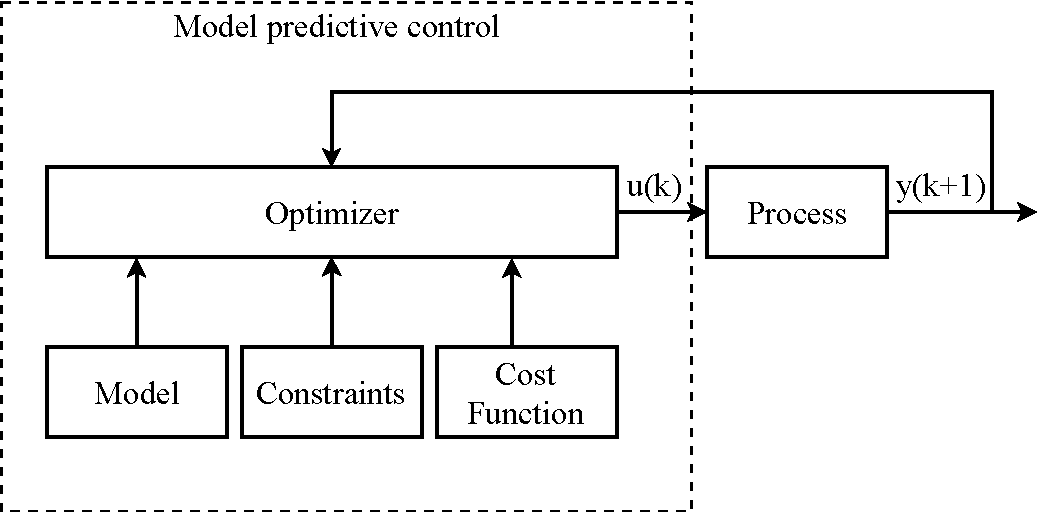
\includegraphics[width=0.60\textwidth]{report/control/pictures/mpc_diagram}
	\caption{Diagram of an MPC controller}
	\label{fig:mpc_diagram}
\end{figure}

Here it is illustrated that the model, constraint and cost function will be used in the optimizer to generate an control output, that will be used in the process, which in this case is the nonlinear model. The output y(k+1) is the output height at the end of the last pipe in the sewer network. At each time step the current value of the output is feedback to the MPC controller. Here the MPC will at each iteration calculate up to $H_p$ control inputs, as it calculates for future disturbances, however, only the first element of this u vector will be used to control the process. Thereafter a new measurement will be taken and a new controller output will be calculated and this will iterate for the entire simulation.

In determining the length of the prediction horizon several considerations were taken into account. As illustration in section \ref{sec:WWTP_challenges} in figure \ref{fig:input_to_wwtp} a daily flow from the households is shown. Here the flow is illustrated for working days and in the weekend. Thereby by knowing the flow pattern for households the MPC would be able to include this knowledge in the prediction model. Thus ideal prediction horizon would be 24 hours, as it would be able to see the disturbance across a whole day. However, as the households are not the only disturbance in this setup this is not entirely true. Because the disturbance coming from the larger industry e.g. the bottling plant and the brewery are stochastic in a way, where it is unknown when the wastewater from the plants is coming and the periodicity between the outlets are unknown. Furthermore, the amount of wastewater coming from the plants are also different from time to time. Therefore, it would not be preferable to place the tank next to the industry as it would not be able to predict the disturbance. Thus the tank needs to be placed in a distance away from the industry, where it would be able to use the disturbance in the prediction model by knowing the disturbance coming from the industry by having a measurement of it. The time it takes the wastewater to leave the industry and to arrive at the tank would then decide the length of the prediction horizon. However, in the implementation of the MPC, it was discovered that the prediction horizon was restricted. Because when it was set to high, above 20, the quadratic $\CMcal{H}$ matrix, equation \ref{eq:quadratic_h_matrix}, was not semi-positive definite, as in the eigenvalues of it was negative, hence the quadratic problem was not convex. The reason for this problem is, that in the linearized model, some of the elements in matrices are very small and therefore, when the system is predicted, as shown in equation \ref{eq:lifted_state_equation}, the elements would be even smaller, thus causing the $\CMcal{H}$ matrix to have an extremely small negative eigenvalue. Therefore, several tests were conducted to find a prediction horizon that did not result in a negative eigenvalue. It was found that a prediction horizon of 20, thereby, the lowest eigenvalue of $\CMcal{H}$ was zero. However, this restricts the length of the pipe after the tank, because if the pipe is too long the MPC will not be able to predict all the way down to the output of it. Therefore, in the simulation of the MPC controller, this must be kept in mind.   

\subsection*{Results}
In the subsection the results obtained from the testing of the MPC controller will be covered. Two simulation will conducted, one where the constraints are neglected and therefore minimized without any restriction and another simulation where the constraints included. 

The pipe and tank setup for the simulation includes two pipes and one tank, where the tank is placed in the middle of the pipes. The specification for both pipes and the tank can be seen in tabular \ref{tab:pipe_data_for_mpc_test} and \ref{tab:tank_data_for_mpc_test} respectively.

\begin{table}[H]
\centering
\begin{tabular}{|c|c|c|c|c|c|c|c|}
\hline
\textbf{Pipe number} & \textbf{Length} [m] & \textbf{Sections} & \textbf{Dx} [m] & \textbf{Ib} & \textbf{d} [m] & \textbf{$\theta$} & \textbf{Qf $[m^3/s]$} \\ \hline
1&100             & 5                 & 20          & 0,003       & 0,9        & 0,65              & 0,97        \\ \hline
2&100             & 5                 & 20          & 0,003       & 0,9        & 0,65              & 0,97        \\ \hline
\end{tabular}
\caption{The pipe specification for the test.}
\label{tab:pipe_data_for_mpc_test}
\end{table}
\begin{table}[H]
\centering
\begin{tabular}{|c|c|}
\hline
\textbf{Size $[m^3]$}        & 90   \\ \hline
\textbf{Height $[m]$}      & 10   \\ \hline
\textbf{Area $[m^2]$}        & 9    \\ \hline
\textbf{Q\_out\_max} $[m^3/s]$& 0,97 \\ \hline
\end{tabular}
\caption{Tank specification for the test.}
\label{tab:tank_data_for_mpc_test}
\end{table}

In the first simulation the MPC controller is minimizing the output variations of the tank without any constraints included. The input signal in the first pipe is shown in figure \ref{fig:input_to_pipe_mpc_test}. 
\begin{figure}[H]
 \centering
 % This file was created by matlab2tikz.
%
%The latest updates can be retrieved from
%  http://www.mathworks.com/matlabcentral/fileexchange/22022-matlab2tikz-matlab2tikz
%where you can also make suggestions and rate matlab2tikz.
%
\definecolor{mycolor1}{rgb}{0.00000,0.44700,0.74100}%
%
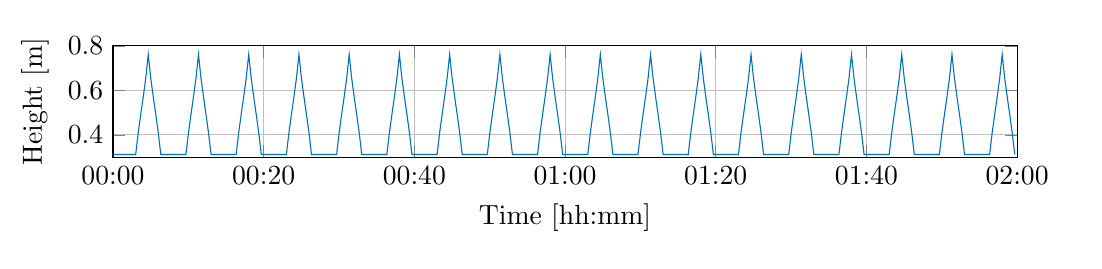
\begin{tikzpicture}
\vspace{5mm}
\hspace{-2mm}
\begin{axis}[%
width=4.521in,
height=.5566in,
at={(0.758in,0.481in)},
scale only axis,
xmin=0,
xmax=7200,
xtick={0,1200,2400,3600,4800,6000,7200},
xticklabels={{00:00},{00:20},{00:40},{01:00},{01:20},{01:40},{02:00},{},{}},
xlabel={Time [hh:mm]},
xmajorgrids,
ymin=0.3,
ymax=0.8,
ylabel={Height [m]},
ymajorgrids,
axis background/.style={fill=white}
]
\addplot [color=mycolor1,solid,forget plot]
  table[row sep=crcr]{%
1	0.31203\\
21	0.31203\\
41	0.31203\\
61	0.31203\\
81	0.31203\\
101	0.31203\\
121	0.31203\\
141	0.31203\\
161	0.31203\\
181	0.31203\\
201	0.40851\\
221	0.49122\\
241	0.57033\\
261	0.65412\\
281	0.76113\\
301	0.65412\\
321	0.57033\\
341	0.49122\\
361	0.40851\\
381	0.31203\\
401	0.31203\\
421	0.31203\\
441	0.31203\\
461	0.31203\\
481	0.31203\\
501	0.31203\\
521	0.31203\\
541	0.31203\\
561	0.31203\\
581	0.31203\\
601	0.40851\\
621	0.49122\\
641	0.57033\\
661	0.65412\\
681	0.76113\\
701	0.65412\\
721	0.57033\\
741	0.49122\\
761	0.40851\\
781	0.31203\\
801	0.31203\\
821	0.31203\\
841	0.31203\\
861	0.31203\\
881	0.31203\\
901	0.31203\\
921	0.31203\\
941	0.31203\\
961	0.31203\\
981	0.31203\\
1001	0.40851\\
1021	0.49122\\
1041	0.57033\\
1061	0.65412\\
1081	0.76113\\
1101	0.65412\\
1121	0.57033\\
1141	0.49122\\
1161	0.40851\\
1181	0.31203\\
1201	0.31203\\
1221	0.31203\\
1241	0.31203\\
1261	0.31203\\
1281	0.31203\\
1301	0.31203\\
1321	0.31203\\
1341	0.31203\\
1361	0.31203\\
1381	0.31203\\
1401	0.40851\\
1421	0.49122\\
1441	0.57033\\
1461	0.65412\\
1481	0.76113\\
1501	0.65412\\
1521	0.57033\\
1541	0.49122\\
1561	0.40851\\
1581	0.31203\\
1601	0.31203\\
1621	0.31203\\
1641	0.31203\\
1661	0.31203\\
1681	0.31203\\
1701	0.31203\\
1721	0.31203\\
1741	0.31203\\
1761	0.31203\\
1781	0.31203\\
1801	0.40851\\
1821	0.49122\\
1841	0.57033\\
1861	0.65412\\
1881	0.76113\\
1901	0.65412\\
1921	0.57033\\
1941	0.49122\\
1961	0.40851\\
1981	0.31203\\
2001	0.31203\\
2021	0.31203\\
2041	0.31203\\
2061	0.31203\\
2081	0.31203\\
2101	0.31203\\
2121	0.31203\\
2141	0.31203\\
2161	0.31203\\
2181	0.31203\\
2201	0.40851\\
2221	0.49122\\
2241	0.57033\\
2261	0.65412\\
2281	0.76113\\
2301	0.65412\\
2321	0.57033\\
2341	0.49122\\
2361	0.40851\\
2381	0.31203\\
2401	0.31203\\
2421	0.31203\\
2441	0.31203\\
2461	0.31203\\
2481	0.31203\\
2501	0.31203\\
2521	0.31203\\
2541	0.31203\\
2561	0.31203\\
2581	0.31203\\
2601	0.40851\\
2621	0.49122\\
2641	0.57033\\
2661	0.65412\\
2681	0.76113\\
2701	0.65412\\
2721	0.57033\\
2741	0.49122\\
2761	0.40851\\
2781	0.31203\\
2801	0.31203\\
2821	0.31203\\
2841	0.31203\\
2861	0.31203\\
2881	0.31203\\
2901	0.31203\\
2921	0.31203\\
2941	0.31203\\
2961	0.31203\\
2981	0.31203\\
3001	0.40851\\
3021	0.49122\\
3041	0.57033\\
3061	0.65412\\
3081	0.76113\\
3101	0.65412\\
3121	0.57033\\
3141	0.49122\\
3161	0.40851\\
3181	0.31203\\
3201	0.31203\\
3221	0.31203\\
3241	0.31203\\
3261	0.31203\\
3281	0.31203\\
3301	0.31203\\
3321	0.31203\\
3341	0.31203\\
3361	0.31203\\
3381	0.31203\\
3401	0.40851\\
3421	0.49122\\
3441	0.57033\\
3461	0.65412\\
3481	0.76113\\
3501	0.65412\\
3521	0.57033\\
3541	0.49122\\
3561	0.40851\\
3581	0.31203\\
3601	0.31203\\
3621	0.31203\\
3641	0.31203\\
3661	0.31203\\
3681	0.31203\\
3701	0.31203\\
3721	0.31203\\
3741	0.31203\\
3761	0.31203\\
3781	0.31203\\
3801	0.40851\\
3821	0.49122\\
3841	0.57033\\
3861	0.65412\\
3881	0.76113\\
3901	0.65412\\
3921	0.57033\\
3941	0.49122\\
3961	0.40851\\
3981	0.31203\\
4001	0.31203\\
4021	0.31203\\
4041	0.31203\\
4061	0.31203\\
4081	0.31203\\
4101	0.31203\\
4121	0.31203\\
4141	0.31203\\
4161	0.31203\\
4181	0.31203\\
4201	0.40851\\
4221	0.49122\\
4241	0.57033\\
4261	0.65412\\
4281	0.76113\\
4301	0.65412\\
4321	0.57033\\
4341	0.49122\\
4361	0.40851\\
4381	0.31203\\
4401	0.31203\\
4421	0.31203\\
4441	0.31203\\
4461	0.31203\\
4481	0.31203\\
4501	0.31203\\
4521	0.31203\\
4541	0.31203\\
4561	0.31203\\
4581	0.31203\\
4601	0.40851\\
4621	0.49122\\
4641	0.57033\\
4661	0.65412\\
4681	0.76113\\
4701	0.65412\\
4721	0.57033\\
4741	0.49122\\
4761	0.40851\\
4781	0.31203\\
4801	0.31203\\
4821	0.31203\\
4841	0.31203\\
4861	0.31203\\
4881	0.31203\\
4901	0.31203\\
4921	0.31203\\
4941	0.31203\\
4961	0.31203\\
4981	0.31203\\
5001	0.40851\\
5021	0.49122\\
5041	0.57033\\
5061	0.65412\\
5081	0.76113\\
5101	0.65412\\
5121	0.57033\\
5141	0.49122\\
5161	0.40851\\
5181	0.31203\\
5201	0.31203\\
5221	0.31203\\
5241	0.31203\\
5261	0.31203\\
5281	0.31203\\
5301	0.31203\\
5321	0.31203\\
5341	0.31203\\
5361	0.31203\\
5381	0.31203\\
5401	0.40851\\
5421	0.49122\\
5441	0.57033\\
5461	0.65412\\
5481	0.76113\\
5501	0.65412\\
5521	0.57033\\
5541	0.49122\\
5561	0.40851\\
5581	0.31203\\
5601	0.31203\\
5621	0.31203\\
5641	0.31203\\
5661	0.31203\\
5681	0.31203\\
5701	0.31203\\
5721	0.31203\\
5741	0.31203\\
5761	0.31203\\
5781	0.31203\\
5801	0.40851\\
5821	0.49122\\
5841	0.57033\\
5861	0.65412\\
5881	0.76113\\
5901	0.65412\\
5921	0.57033\\
5941	0.49122\\
5961	0.40851\\
5981	0.31203\\
6001	0.31203\\
6021	0.31203\\
6041	0.31203\\
6061	0.31203\\
6081	0.31203\\
6101	0.31203\\
6121	0.31203\\
6141	0.31203\\
6161	0.31203\\
6181	0.31203\\
6201	0.40851\\
6221	0.49122\\
6241	0.57033\\
6261	0.65412\\
6281	0.76113\\
6301	0.65412\\
6321	0.57033\\
6341	0.49122\\
6361	0.40851\\
6381	0.31203\\
6401	0.31203\\
6421	0.31203\\
6441	0.31203\\
6461	0.31203\\
6481	0.31203\\
6501	0.31203\\
6521	0.31203\\
6541	0.31203\\
6561	0.31203\\
6581	0.31203\\
6601	0.40851\\
6621	0.49122\\
6641	0.57033\\
6661	0.65412\\
6681	0.76113\\
6701	0.65412\\
6721	0.57033\\
6741	0.49122\\
6761	0.40851\\
6781	0.31203\\
6801	0.31203\\
6821	0.31203\\
6841	0.31203\\
6861	0.31203\\
6881	0.31203\\
6901	0.31203\\
6921	0.31203\\
6941	0.31203\\
6961	0.31203\\
6981	0.31203\\
7001	0.40851\\
7021	0.49122\\
7041	0.57033\\
7061	0.65412\\
7081	0.76113\\
7101	0.65412\\
7121	0.57033\\
7141	0.49122\\
7161	0.40851\\
7181	0.31203\\
};
\end{axis}
\end{tikzpicture}%
\caption{The input to the first pipe.}
\label{fig:input_to_pipe_mpc_test}
\end{figure}

Here there is a constant input of 0,2 $m^3/s$, which results in a height of 0,31 meters in the pipe. On top of the input a disturbance signal is added. This is done to see if the MPC is able to keep the flow variations out of the tank to a minimum. This signal is a upper triangular signal which goes from the constant input up to 0,9 $m^3/s$ which is equal to a height of 0,75 meters in the pipe. The time between each disturbance signal is 200 seconds and the period of the triangle signal is 100 seconds. This simulation conducted for two hours where $\Delta t$ is 20 seconds. In figure \ref{fig:MPC_test_output_first_test} the output of the the last pipe is shown.  


\begin{figure}[H]
 \centering
 % This file was created by matlab2tikz.
%
%The latest updates can be retrieved from
%  http://www.mathworks.com/matlabcentral/fileexchange/22022-matlab2tikz-matlab2tikz
%where you can also make suggestions and rate matlab2tikz.
%
\definecolor{mycolor1}{rgb}{0.00000,0.44700,0.74100}%
%
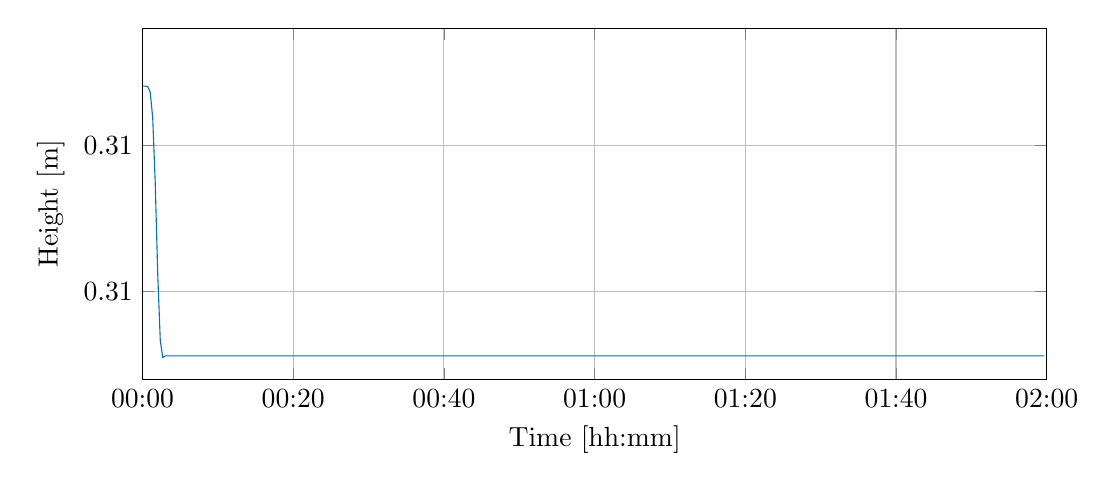
\begin{tikzpicture}

\begin{axis}[%
width=4.521in,
height=1.7566in,
at={(0.758in,0.481in)},
scale only axis,
xmin=0,
xmax=7200,
xtick={0,1200,2400,3600,4800,6000,7200},
xticklabels={{00:00},{00:20},{00:40},{01:00},{01:20},{01:40},{02:00},{},{}},
xlabel={Time [hh:mm]},
xmajorgrids,
ymin=0.302,
ymax=0.314,
ylabel={Height [m]},
ymajorgrids,
axis background/.style={fill=white}
]
\addplot [color=mycolor1,solid,forget plot]
  table[row sep=crcr]{%
1	0.312023251728134\\
21	0.312023249248491\\
41	0.312007329576048\\
61	0.311822355594219\\
81	0.310938012057319\\
101	0.308710026090253\\
121	0.305594844450276\\
141	0.303344739104071\\
161	0.302753859420006\\
181	0.302809429127008\\
201	0.30280716177161\\
221	0.302807232518793\\
241	0.302807230514799\\
261	0.302807230566105\\
281	0.30280723056466\\
301	0.302807230564718\\
321	0.302807230564717\\
341	0.302807230564717\\
361	0.302807230564717\\
381	0.302807230564717\\
401	0.302807230564717\\
421	0.302807230564717\\
441	0.302807230564717\\
461	0.302807230564717\\
481	0.302807230564717\\
501	0.302807230564717\\
521	0.302807230564717\\
541	0.302807230564717\\
561	0.302807230564717\\
581	0.302807230564717\\
601	0.302807230564717\\
621	0.302807230564717\\
641	0.302807230564717\\
661	0.302807230564717\\
681	0.302807230564717\\
701	0.302807230564717\\
721	0.302807230564717\\
741	0.302807230564717\\
761	0.302807230564717\\
781	0.302807230564717\\
801	0.302807230564717\\
821	0.302807230564717\\
841	0.302807230564717\\
861	0.302807230564717\\
881	0.302807230564717\\
901	0.302807230564717\\
921	0.302807230564717\\
941	0.302807230564717\\
961	0.302807230564717\\
981	0.302807230564717\\
1001	0.302807230564717\\
1021	0.302807230564717\\
1041	0.302807230564717\\
1061	0.302807230564717\\
1081	0.302807230564717\\
1101	0.302807230564717\\
1121	0.302807230564717\\
1141	0.302807230564717\\
1161	0.302807230564717\\
1181	0.302807230564717\\
1201	0.302807230564717\\
1221	0.302807230564717\\
1241	0.302807230564717\\
1261	0.302807230564717\\
1281	0.302807230564717\\
1301	0.302807230564717\\
1321	0.302807230564717\\
1341	0.302807230564717\\
1361	0.302807230564717\\
1381	0.302807230564717\\
1401	0.302807230564717\\
1421	0.302807230564717\\
1441	0.302807230564717\\
1461	0.302807230564717\\
1481	0.302807230564717\\
1501	0.302807230564717\\
1521	0.302807230564717\\
1541	0.302807230564717\\
1561	0.302807230564717\\
1581	0.302807230564717\\
1601	0.302807230564717\\
1621	0.302807230564717\\
1641	0.302807230564717\\
1661	0.302807230564717\\
1681	0.302807230564717\\
1701	0.302807230564717\\
1721	0.302807230564717\\
1741	0.302807230564717\\
1761	0.302807230564717\\
1781	0.302807230564717\\
1801	0.302807230564717\\
1821	0.302807230564717\\
1841	0.302807230564717\\
1861	0.302807230564717\\
1881	0.302807230564717\\
1901	0.302807230564717\\
1921	0.302807230564717\\
1941	0.302807230564717\\
1961	0.302807230564717\\
1981	0.302807230564717\\
2001	0.302807230564717\\
2021	0.302807230564717\\
2041	0.302807230564717\\
2061	0.302807230564717\\
2081	0.302807230564717\\
2101	0.302807230564717\\
2121	0.302807230564717\\
2141	0.302807230564717\\
2161	0.302807230564717\\
2181	0.302807230564717\\
2201	0.302807230564717\\
2221	0.302807230564717\\
2241	0.302807230564717\\
2261	0.302807230564717\\
2281	0.302807230564717\\
2301	0.302807230564717\\
2321	0.302807230564717\\
2341	0.302807230564717\\
2361	0.302807230564717\\
2381	0.302807230564717\\
2401	0.302807230564717\\
2421	0.302807230564717\\
2441	0.302807230564717\\
2461	0.302807230564717\\
2481	0.302807230564717\\
2501	0.302807230564717\\
2521	0.302807230564717\\
2541	0.302807230564717\\
2561	0.302807230564717\\
2581	0.302807230564717\\
2601	0.302807230564717\\
2621	0.302807230564717\\
2641	0.302807230564717\\
2661	0.302807230564717\\
2681	0.302807230564717\\
2701	0.302807230564717\\
2721	0.302807230564717\\
2741	0.302807230564717\\
2761	0.302807230564717\\
2781	0.302807230564717\\
2801	0.302807230564717\\
2821	0.302807230564717\\
2841	0.302807230564717\\
2861	0.302807230564717\\
2881	0.302807230564717\\
2901	0.302807230564717\\
2921	0.302807230564717\\
2941	0.302807230564717\\
2961	0.302807230564717\\
2981	0.302807230564717\\
3001	0.302807230564717\\
3021	0.302807230564717\\
3041	0.302807230564717\\
3061	0.302807230564717\\
3081	0.302807230564717\\
3101	0.302807230564717\\
3121	0.302807230564717\\
3141	0.302807230564717\\
3161	0.302807230564717\\
3181	0.302807230564717\\
3201	0.302807230564717\\
3221	0.302807230564717\\
3241	0.302807230564717\\
3261	0.302807230564717\\
3281	0.302807230564717\\
3301	0.302807230564717\\
3321	0.302807230564717\\
3341	0.302807230564717\\
3361	0.302807230564717\\
3381	0.302807230564717\\
3401	0.302807230564717\\
3421	0.302807230564717\\
3441	0.302807230564717\\
3461	0.302807230564717\\
3481	0.302807230564717\\
3501	0.302807230564717\\
3521	0.302807230564717\\
3541	0.302807230564717\\
3561	0.302807230564717\\
3581	0.302807230564717\\
3601	0.302807230564717\\
3621	0.302807230564717\\
3641	0.302807230564717\\
3661	0.302807230564717\\
3681	0.302807230564717\\
3701	0.302807230564717\\
3721	0.302807230564717\\
3741	0.302807230564717\\
3761	0.302807230564717\\
3781	0.302807230564717\\
3801	0.302807230564717\\
3821	0.302807230564717\\
3841	0.302807230564717\\
3861	0.302807230564717\\
3881	0.302807230564717\\
3901	0.302807230564717\\
3921	0.302807230564717\\
3941	0.302807230564717\\
3961	0.302807230564717\\
3981	0.302807230564717\\
4001	0.302807230564717\\
4021	0.302807230564717\\
4041	0.302807230564717\\
4061	0.302807230564717\\
4081	0.302807230564717\\
4101	0.302807230564717\\
4121	0.302807230564717\\
4141	0.302807230564717\\
4161	0.302807230564717\\
4181	0.302807230564717\\
4201	0.302807230564717\\
4221	0.302807230564717\\
4241	0.302807230564717\\
4261	0.302807230564717\\
4281	0.302807230564717\\
4301	0.302807230564717\\
4321	0.302807230564717\\
4341	0.302807230564717\\
4361	0.302807230564717\\
4381	0.302807230564717\\
4401	0.302807230564717\\
4421	0.302807230564717\\
4441	0.302807230564717\\
4461	0.302807230564717\\
4481	0.302807230564717\\
4501	0.302807230564717\\
4521	0.302807230564717\\
4541	0.302807230564717\\
4561	0.302807230564717\\
4581	0.302807230564717\\
4601	0.302807230564717\\
4621	0.302807230564717\\
4641	0.302807230564717\\
4661	0.302807230564717\\
4681	0.302807230564717\\
4701	0.302807230564717\\
4721	0.302807230564717\\
4741	0.302807230564717\\
4761	0.302807230564717\\
4781	0.302807230564717\\
4801	0.302807230564717\\
4821	0.302807230564717\\
4841	0.302807230564717\\
4861	0.302807230564717\\
4881	0.302807230564717\\
4901	0.302807230564717\\
4921	0.302807230564717\\
4941	0.302807230564717\\
4961	0.302807230564717\\
4981	0.302807230564717\\
5001	0.302807230564717\\
5021	0.302807230564717\\
5041	0.302807230564717\\
5061	0.302807230564717\\
5081	0.302807230564717\\
5101	0.302807230564717\\
5121	0.302807230564717\\
5141	0.302807230564717\\
5161	0.302807230564717\\
5181	0.302807230564717\\
5201	0.302807230564717\\
5221	0.302807230564717\\
5241	0.302807230564717\\
5261	0.302807230564717\\
5281	0.302807230564717\\
5301	0.302807230564717\\
5321	0.302807230564717\\
5341	0.302807230564717\\
5361	0.302807230564717\\
5381	0.302807230564717\\
5401	0.302807230564717\\
5421	0.302807230564717\\
5441	0.302807230564717\\
5461	0.302807230564717\\
5481	0.302807230564717\\
5501	0.302807230564717\\
5521	0.302807230564717\\
5541	0.302807230564717\\
5561	0.302807230564717\\
5581	0.302807230564717\\
5601	0.302807230564717\\
5621	0.302807230564717\\
5641	0.302807230564717\\
5661	0.302807230564717\\
5681	0.302807230564717\\
5701	0.302807230564717\\
5721	0.302807230564717\\
5741	0.302807230564717\\
5761	0.302807230564717\\
5781	0.302807230564717\\
5801	0.302807230564717\\
5821	0.302807230564717\\
5841	0.302807230564717\\
5861	0.302807230564717\\
5881	0.302807230564717\\
5901	0.302807230564717\\
5921	0.302807230564717\\
5941	0.302807230564717\\
5961	0.302807230564717\\
5981	0.302807230564717\\
6001	0.302807230564717\\
6021	0.302807230564717\\
6041	0.302807230564717\\
6061	0.302807230564717\\
6081	0.302807230564717\\
6101	0.302807230564717\\
6121	0.302807230564717\\
6141	0.302807230564717\\
6161	0.302807230564717\\
6181	0.302807230564717\\
6201	0.302807230564717\\
6221	0.302807230564717\\
6241	0.302807230564717\\
6261	0.302807230564717\\
6281	0.302807230564717\\
6301	0.302807230564717\\
6321	0.302807230564717\\
6341	0.302807230564717\\
6361	0.302807230564717\\
6381	0.302807230564717\\
6401	0.302807230564717\\
6421	0.302807230564717\\
6441	0.302807230564717\\
6461	0.302807230564717\\
6481	0.302807230564717\\
6501	0.302807230564717\\
6521	0.302807230564717\\
6541	0.302807230564717\\
6561	0.302807230564717\\
6581	0.302807230564717\\
6601	0.302807230564717\\
6621	0.302807230564717\\
6641	0.302807230564717\\
6661	0.302807230564717\\
6681	0.302807230564717\\
6701	0.302807230564717\\
6721	0.302807230564717\\
6741	0.302807230564717\\
6761	0.302807230564717\\
6781	0.302807230564717\\
6801	0.302807230564717\\
6821	0.302807230564717\\
6841	0.302807230564717\\
6861	0.302807230564717\\
6881	0.302807230564717\\
6901	0.302807230564717\\
6921	0.302807230564717\\
6941	0.302807230564717\\
6961	0.302807230564717\\
6981	0.302807230564717\\
7001	0.302807230564717\\
7021	0.302807230564717\\
7041	0.302807230564717\\
7061	0.302807230564717\\
7081	0.302807230564717\\
7101	0.302807230564717\\
7121	0.302807230564717\\
7141	0.302807230564717\\
7161	0.302807230564717\\
7181	0.302807230564717\\
};
\end{axis}
\end{tikzpicture}%
\caption{The output of the last pipe.}
\label{fig:MPC_test_output_first_test}
\end{figure}

Here it can be seen that the MPC controller is able to minimize the disturbance coming from the first pipe as the output is constant. At the beginning the height of the output is a bit higher, this is due to that the tank holds wastewater at the beginning of the simulation. After it is emptied the height falls down to a constant level. In figure \ref{fig:tank_height_first_test} the height in the tank can be seen.  

\begin{figure}[H]
 \centering
 % This file was created by matlab2tikz.
%
%The latest updates can be retrieved from
%  http://www.mathworks.com/matlabcentral/fileexchange/22022-matlab2tikz-matlab2tikz
%where you can also make suggestions and rate matlab2tikz.
%
\definecolor{mycolor1}{rgb}{0.00000,0.44700,0.74100}%
%
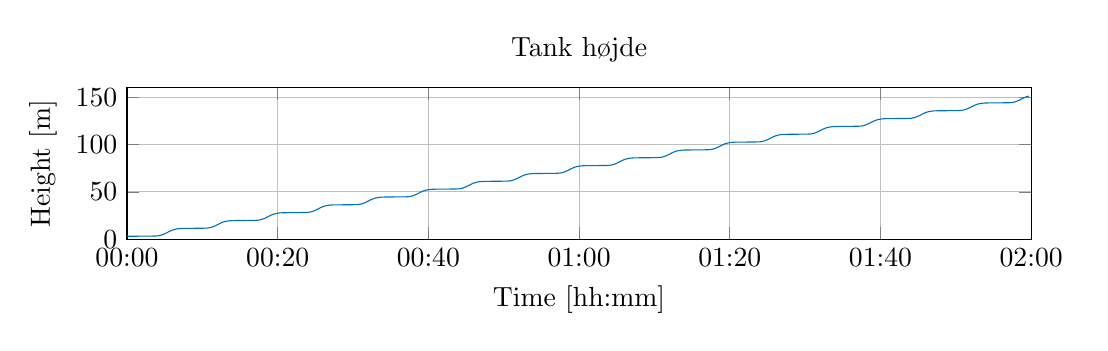
\begin{tikzpicture}
\hspace{-1mm}
\begin{axis}[%
width=4.521in,
height=.7566in,
at={(0.758in,0.481in)},
scale only axis,
xmin=0,
xmax=7200,
title ={Tank højde},
xtick={0,1200,2400,3600,4800,6000,7200},
xticklabels={{00:00},{00:20},{00:40},{01:00},{01:20},{01:40},{02:00},{},{}},
xlabel={Time [hh:mm]},
xmajorgrids,
ymin=-0.1,
ymax=160,
ylabel={Height [m]},
ymajorgrids,
axis background/.style={fill=white}
]
\addplot [color=mycolor1,solid,forget plot]
  table[row sep=crcr]{%
1	3\\
21	2.99999999316026\\
41	3.01333332012207\\
61	3.03959998125893\\
81	3.06547864251583\\
101	3.0913689429355\\
121	3.11725889387259\\
141	3.14314885534856\\
161	3.16903881650788\\
181	3.19492877767658\\
201	3.22208190892336\\
221	3.26581919849303\\
241	3.40261431116685\\
261	3.80277617108737\\
281	4.582895898918\\
301	5.68730591534825\\
321	7.00239347163539\\
341	8.36007404320854\\
361	9.51275135815108\\
381	10.3267153588503\\
401	10.8543133136161\\
421	11.1590600902295\\
441	11.2945893110534\\
461	11.3388672109703\\
481	11.3608410656606\\
501	11.3869549591855\\
521	11.4128355845539\\
541	11.4387258658624\\
561	11.4646158173399\\
581	11.4905057788189\\
601	11.5176589100695\\
621	11.5613961996392\\
641	11.698191312313\\
661	12.0983531722335\\
681	12.8784729000642\\
701	13.9828829164944\\
721	15.2979704727815\\
741	16.6556510443547\\
761	17.8083283592972\\
781	18.6222923599965\\
801	19.1498903147623\\
821	19.4546370913756\\
841	19.5901663121995\\
861	19.6344442121164\\
881	19.6564180668067\\
901	19.6825319603317\\
921	19.7084125857001\\
941	19.7343028670085\\
961	19.7601928184861\\
981	19.7860827799651\\
1001	19.8132359112157\\
1021	19.8569732007853\\
1041	19.9937683134592\\
1061	20.3939301733797\\
1081	21.1740499012103\\
1101	22.2784599176406\\
1121	23.5935474739277\\
1141	24.9512280455008\\
1161	26.1039053604434\\
1181	26.9178693611426\\
1201	27.4454673159084\\
1221	27.7502140925218\\
1241	27.8857433133457\\
1261	27.9300212132626\\
1281	27.9519950679529\\
1301	27.9781089614778\\
1321	28.0039895868462\\
1341	28.0298798681547\\
1361	28.0557698196322\\
1381	28.0816597811112\\
1401	28.1088129123618\\
1421	28.1525502019315\\
1441	28.2893453146053\\
1461	28.6895071745258\\
1481	29.4696269023564\\
1501	30.5740369187867\\
1521	31.8891244750738\\
1541	33.246805046647\\
1561	34.3994823615895\\
1581	35.2134463622888\\
1601	35.7410443170546\\
1621	36.0457910936679\\
1641	36.1813203144918\\
1661	36.2255982144087\\
1681	36.247572069099\\
1701	36.273685962624\\
1721	36.2995665879924\\
1741	36.3254568693008\\
1761	36.3513468207784\\
1781	36.3772367822573\\
1801	36.404389913508\\
1821	36.4481272030776\\
1841	36.5849223157514\\
1861	36.985084175672\\
1881	37.7652039035026\\
1901	38.8696139199329\\
1921	40.18470147622\\
1941	41.5423820477931\\
1961	42.6950593627357\\
1981	43.5090233634349\\
2001	44.0366213182008\\
2021	44.3413680948141\\
2041	44.476897315638\\
2061	44.5211752155549\\
2081	44.5431490702452\\
2101	44.5692629637701\\
2121	44.5951435891385\\
2141	44.621033870447\\
2161	44.6469238219245\\
2181	44.6728137834035\\
2201	44.6999669146541\\
2221	44.7437042042238\\
2241	44.8804993168976\\
2261	45.2806611768181\\
2281	46.0607809046488\\
2301	47.165190921079\\
2321	48.4802784773661\\
2341	49.8379590489393\\
2361	50.9906363638818\\
2381	51.8046003645811\\
2401	52.3321983193469\\
2421	52.6369450959602\\
2441	52.7724743167841\\
2461	52.816752216701\\
2481	52.8387260713913\\
2501	52.8648399649163\\
2521	52.8907205902847\\
2541	52.9166108715932\\
2561	52.9425008230707\\
2581	52.9683907845497\\
2601	52.9955439158003\\
2621	53.0392812053699\\
2641	53.1760763180438\\
2661	53.5762381779643\\
2681	54.3563579057949\\
2701	55.4607679222252\\
2721	56.7758554785123\\
2741	58.1335360500855\\
2761	59.286213365028\\
2781	60.1001773657272\\
2801	60.6277753204931\\
2821	60.9325220971064\\
2841	61.0680513179303\\
2861	61.1123292178472\\
2881	61.1343030725375\\
2901	61.1604169660624\\
2921	61.1862975914308\\
2941	61.2121878727393\\
2961	61.2380778242168\\
2981	61.2639677856958\\
3001	61.2911209169465\\
3021	61.3348582065161\\
3041	61.4716533191899\\
3061	61.8718151791104\\
3081	62.6519349069411\\
3101	63.7563449233713\\
3121	65.0714324796585\\
3141	66.4291130512316\\
3161	67.5817903661741\\
3181	68.3957543668734\\
3201	68.9233523216392\\
3221	69.2280990982525\\
3241	69.3636283190764\\
3261	69.4079062189933\\
3281	69.4298800736836\\
3301	69.4559939672086\\
3321	69.481874592577\\
3341	69.5077648738854\\
3361	69.533654825363\\
3381	69.559544786842\\
3401	69.5866979180926\\
3421	69.6304352076622\\
3441	69.7672303203361\\
3461	70.1673921802566\\
3481	70.9475119080872\\
3501	72.0519219245175\\
3521	73.3670094808046\\
3541	74.7246900523778\\
3561	75.8773673673203\\
3581	76.6913313680195\\
3601	77.2189293227854\\
3621	77.5236760993987\\
3641	77.6592053202226\\
3661	77.7034832201395\\
3681	77.7254570748298\\
3701	77.7515709683547\\
3721	77.7774515937231\\
3741	77.8033418750316\\
3761	77.8292318265091\\
3781	77.8551217879881\\
3801	77.8822749192387\\
3821	77.9260122088084\\
3841	78.0628073214822\\
3861	78.4629691814027\\
3881	79.2430889092334\\
3901	80.3474989256636\\
3921	81.6625864819507\\
3941	83.0202670535239\\
3961	84.1729443684664\\
3981	84.9869083691657\\
4001	85.5145063239315\\
4021	85.8192531005448\\
4041	85.9547823213687\\
4061	85.9990602212856\\
4081	86.0210340759759\\
4101	86.0471479695009\\
4121	86.0730285948693\\
4141	86.0989188761777\\
4161	86.1248088276553\\
4181	86.1506987891342\\
4201	86.1778519203849\\
4221	86.2215892099545\\
4241	86.3583843226283\\
4261	86.7585461825489\\
4281	87.5386659103795\\
4301	88.6430759268097\\
4321	89.9581634830969\\
4341	91.31584405467\\
4361	92.4685213696126\\
4381	93.2824853703118\\
4401	93.8100833250776\\
4421	94.114830101691\\
4441	94.2503593225149\\
4461	94.2946372224318\\
4481	94.3166110771221\\
4501	94.342724970647\\
4521	94.3686055960154\\
4541	94.3944958773239\\
4561	94.4203858288014\\
4581	94.4462757902804\\
4601	94.473428921531\\
4621	94.5171662111007\\
4641	94.6539613237745\\
4661	95.054123183695\\
4681	95.8342429115256\\
4701	96.9386529279559\\
4721	98.253740484243\\
4741	99.6114210558162\\
4761	100.764098370759\\
4781	101.578062371458\\
4801	102.105660326224\\
4821	102.410407102837\\
4841	102.545936323661\\
4861	102.590214223578\\
4881	102.612188078268\\
4901	102.638301971793\\
4921	102.664182597162\\
4941	102.69007287847\\
4961	102.715962829948\\
4981	102.741852791427\\
5001	102.769005922677\\
5021	102.812743212247\\
5041	102.949538324921\\
5061	103.349700184841\\
5081	104.129819912672\\
5101	105.234229929102\\
5121	106.549317485389\\
5141	107.906998056962\\
5161	109.059675371905\\
5181	109.873639372604\\
5201	110.40123732737\\
5221	110.705984103983\\
5241	110.841513324807\\
5261	110.885791224724\\
5281	110.907765079414\\
5301	110.933878972939\\
5321	110.959759598308\\
5341	110.985649879616\\
5361	111.011539831094\\
5381	111.037429792573\\
5401	111.064582923823\\
5421	111.108320213393\\
5441	111.245115326067\\
5461	111.645277185987\\
5481	112.425396913818\\
5501	113.529806930248\\
5521	114.844894486535\\
5541	116.202575058108\\
5561	117.355252373051\\
5581	118.16921637375\\
5601	118.696814328516\\
5621	119.001561105129\\
5641	119.137090325953\\
5661	119.18136822587\\
5681	119.203342080561\\
5701	119.229455974085\\
5721	119.255336599454\\
5741	119.281226880762\\
5761	119.30711683224\\
5781	119.333006793719\\
5801	119.360159924969\\
5821	119.403897214539\\
5841	119.540692327213\\
5861	119.940854187133\\
5881	120.720973914964\\
5901	121.825383931394\\
5921	123.140471487681\\
5941	124.498152059255\\
5961	125.650829374197\\
5981	126.464793374896\\
6001	126.992391329662\\
6021	127.297138106276\\
6041	127.432667327099\\
6061	127.476945227016\\
6081	127.498919081707\\
6101	127.525032975232\\
6121	127.5509136006\\
6141	127.576803881908\\
6161	127.602693833386\\
6181	127.628583794865\\
6201	127.655736926116\\
6221	127.699474215685\\
6241	127.836269328359\\
6261	128.23643118828\\
6281	129.01655091611\\
6301	130.12096093254\\
6321	131.436048488828\\
6341	132.793729060401\\
6361	133.946406375343\\
6381	134.760370376042\\
6401	135.287968330808\\
6421	135.592715107422\\
6441	135.728244328246\\
6461	135.772522228162\\
6481	135.794496082853\\
6501	135.820609976378\\
6521	135.846490601746\\
6541	135.872380883055\\
6561	135.898270834532\\
6581	135.924160796011\\
6601	135.951313927262\\
6621	135.995051216831\\
6641	136.131846329505\\
6661	136.532008189426\\
6681	137.312127917256\\
6701	138.416537933687\\
6721	139.731625489974\\
6741	141.089306061547\\
6761	142.241983376489\\
6781	143.055947377189\\
6801	143.583545331955\\
6821	143.888292108568\\
6841	144.023821329392\\
6861	144.068099229309\\
6881	144.090073083999\\
6901	144.116186977524\\
6921	144.142067602892\\
6941	144.167957884201\\
6961	144.193847835678\\
6981	144.219737797157\\
7001	144.246890928408\\
7021	144.290628217978\\
7041	144.427423330651\\
7061	144.827585190572\\
7081	145.607704918403\\
7101	146.712114934833\\
7121	148.02720249112\\
7141	149.384883062693\\
7161	150.537560377636\\
7181	151.351524378335\\
};
\end{axis}
\end{tikzpicture}%
\caption{The height in the tank.}
\label{fig:tank_height_first_test}
\end{figure}

As expected the tank would be overfilled, as the disturbance coming from the first pipe is much higher than the output of the second. However, the cost function does what is expected, as it keeps a steady output of the tank and has no knowledge about the limitations of the tank and therefore overfills it. In the second simulation the same input is applied to the first pipe, where the constraints shown in equation \ref{eq:constriants_eq} is utilized. In this simulation only constraints regarding the tank and the control input to the pump have constraints in this system setup. The reason for not having constraints on the heights in the second pipe is, it should be sufficient to have on the control input to the pump, as it will only allow inputs between 0 to 1, where the constant is multiplied on the maximum flow that the second pipe can transfer and thereby not allowing flows higher than that. Furthermore, the constraints for the tank goes from 0 to the maximum height it, which is 10 meters in this simulation seen in table \ref{tab:tank_data_for_mpc_test}. The reason for not have constraints on the first pipe is, as it is impossible for the MPC controller to regulate the height in that part, therefore the input to the first pipe must so it does not overfills or goes below zero. In figure \ref{fig:tank_height_second_test_with_constraints} the height of the tank is shown from the second simulation.        


\begin{figure}[H]
 \centering
 % This file was created by matlab2tikz.
%
%The latest updates can be retrieved from
%  http://www.mathworks.com/matlabcentral/fileexchange/22022-matlab2tikz-matlab2tikz
%where you can also make suggestions and rate matlab2tikz.
%
\definecolor{mycolor1}{rgb}{0.00000,0.44700,0.74100}%
%
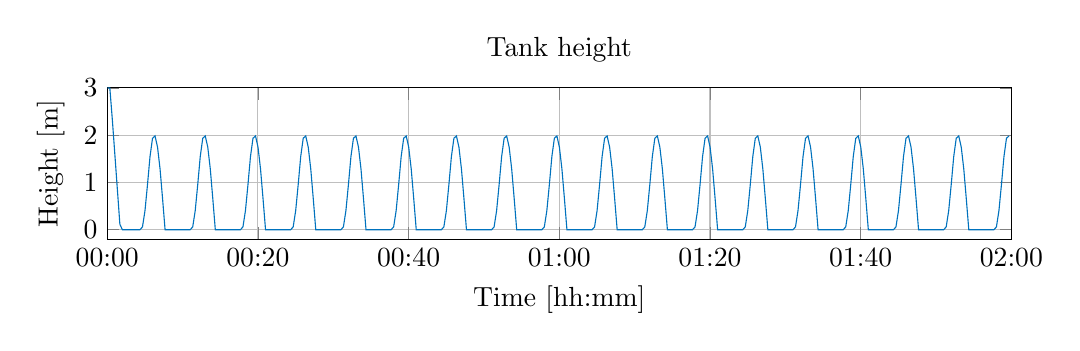
\begin{tikzpicture}

\begin{axis}[%
width=4.521in,
height=.7566in,
/pgf/number format/1000 sep={.},/pgf/number format/use comma,
at={(0.758in,0.481in)},
scale only axis,
xmin=0,
title={Tank height},
xmax=7200,
xtick={0,1200,2400,3600,4800,6000,7200},
xticklabels={{00:00},{00:20},{00:40},{01:00},{01:20},{01:40},{02:00},{},{}},
xlabel={Time [hh:mm]},
xmajorgrids,
ymin=-0.2,
ymax=3,
ylabel={Height [m]},
ymajorgrids,
axis background/.style={fill=white}
]
\addplot [color=mycolor1,solid,forget plot]
  table[row sep=crcr]{%
1	3\\
21	2.99999999316026\\
41	2.32754415169987\\
61	1.59384668206183\\
81	0.855486505639804\\
101	0.11665418915018\\
121	0\\
141	0\\
161	0\\
181	0\\
201	0\\
221	0\\
241	0\\
261	0\\
281	0.0595953504678914\\
301	0.40302542412948\\
321	0.953696376221655\\
341	1.54661857226603\\
361	1.93450659540532\\
381	1.98368241475169\\
401	1.74649216864076\\
421	1.28645074216793\\
441	0.6571917603094\\
461	0\\
481	0\\
501	0\\
521	0\\
541	0\\
561	0\\
581	0\\
601	0\\
621	0\\
641	0\\
661	0\\
681	0.0595953504680377\\
701	0.403025424129614\\
721	0.953696376221789\\
741	1.54661857226616\\
761	1.93450659540545\\
781	1.98368241475182\\
801	1.74649216864089\\
821	1.28645074216806\\
841	0.657191760309528\\
861	0\\
881	0\\
901	0\\
921	0\\
941	0\\
961	0\\
981	0\\
1001	0\\
1021	0\\
1041	0\\
1061	0\\
1081	0.0595953504680377\\
1101	0.403025424129614\\
1121	0.953696376221789\\
1141	1.54661857226616\\
1161	1.93450659540545\\
1181	1.98368241475182\\
1201	1.74649216864089\\
1221	1.28645074216806\\
1241	0.657191760309528\\
1261	0\\
1281	0\\
1301	0\\
1321	0\\
1341	0\\
1361	0\\
1381	0\\
1401	0\\
1421	0\\
1441	0\\
1461	0\\
1481	0.0595953504680377\\
1501	0.403025424129614\\
1521	0.953696376221789\\
1541	1.54661857226616\\
1561	1.93450659540545\\
1581	1.98368241475182\\
1601	1.74649216864089\\
1621	1.28645074216806\\
1641	0.657191760309528\\
1661	0\\
1681	0\\
1701	0\\
1721	0\\
1741	0\\
1761	0\\
1781	0\\
1801	0\\
1821	0\\
1841	0\\
1861	0\\
1881	0.0595953504680377\\
1901	0.403025424129614\\
1921	0.953696376221789\\
1941	1.54661857226616\\
1961	1.93450659540545\\
1981	1.98368241475182\\
2001	1.74649216864089\\
2021	1.28645074216806\\
2041	0.657191760309528\\
2061	0\\
2081	0\\
2101	0\\
2121	0\\
2141	0\\
2161	0\\
2181	0\\
2201	0\\
2221	0\\
2241	0\\
2261	0\\
2281	0.0595953504680377\\
2301	0.403025424129614\\
2321	0.953696376221789\\
2341	1.54661857226616\\
2361	1.93450659540545\\
2381	1.98368241475182\\
2401	1.74649216864089\\
2421	1.28645074216806\\
2441	0.657191760309528\\
2461	0\\
2481	0\\
2501	0\\
2521	0\\
2541	0\\
2561	0\\
2581	0\\
2601	0\\
2621	0\\
2641	0\\
2661	0\\
2681	0.0595953504680377\\
2701	0.403025424129614\\
2721	0.953696376221789\\
2741	1.54661857226616\\
2761	1.93450659540545\\
2781	1.98368241475182\\
2801	1.74649216864089\\
2821	1.28645074216806\\
2841	0.657191760309528\\
2861	0\\
2881	0\\
2901	0\\
2921	0\\
2941	0\\
2961	0\\
2981	0\\
3001	0\\
3021	0\\
3041	0\\
3061	0\\
3081	0.0595953504680377\\
3101	0.403025424129614\\
3121	0.953696376221789\\
3141	1.54661857226616\\
3161	1.93450659540545\\
3181	1.98368241475182\\
3201	1.74649216864089\\
3221	1.28645074216806\\
3241	0.657191760309528\\
3261	0\\
3281	0\\
3301	0\\
3321	0\\
3341	0\\
3361	0\\
3381	0\\
3401	0\\
3421	0\\
3441	0\\
3461	0\\
3481	0.0595953504680377\\
3501	0.403025424129614\\
3521	0.953696376221789\\
3541	1.54661857226616\\
3561	1.93450659540545\\
3581	1.98368241475182\\
3601	1.74649216864089\\
3621	1.28645074216806\\
3641	0.657191760309528\\
3661	0\\
3681	0\\
3701	0\\
3721	0\\
3741	0\\
3761	0\\
3781	0\\
3801	0\\
3821	0\\
3841	0\\
3861	0\\
3881	0.0595953504680377\\
3901	0.403025424129614\\
3921	0.953696376221789\\
3941	1.54661857226616\\
3961	1.93450659540545\\
3981	1.98368241475182\\
4001	1.74649216864089\\
4021	1.28645074216806\\
4041	0.657191760309528\\
4061	0\\
4081	0\\
4101	0\\
4121	0\\
4141	0\\
4161	0\\
4181	0\\
4201	0\\
4221	0\\
4241	0\\
4261	0\\
4281	0.0595953504680377\\
4301	0.403025424129614\\
4321	0.953696376221789\\
4341	1.54661857226616\\
4361	1.93450659540545\\
4381	1.98368241475182\\
4401	1.74649216864089\\
4421	1.28645074216806\\
4441	0.657191760309528\\
4461	0\\
4481	0\\
4501	0\\
4521	0\\
4541	0\\
4561	0\\
4581	0\\
4601	0\\
4621	0\\
4641	0\\
4661	0\\
4681	0.0595953504680377\\
4701	0.403025424129614\\
4721	0.953696376221789\\
4741	1.54661857226616\\
4761	1.93450659540545\\
4781	1.98368241475182\\
4801	1.74649216864089\\
4821	1.28645074216806\\
4841	0.657191760309528\\
4861	0\\
4881	0\\
4901	0\\
4921	0\\
4941	0\\
4961	0\\
4981	0\\
5001	0\\
5021	0\\
5041	0\\
5061	0\\
5081	0.0595953504680377\\
5101	0.403025424129614\\
5121	0.953696376221789\\
5141	1.54661857226616\\
5161	1.93450659540545\\
5181	1.98368241475182\\
5201	1.74649216864089\\
5221	1.28645074216806\\
5241	0.657191760309528\\
5261	0\\
5281	0\\
5301	0\\
5321	0\\
5341	0\\
5361	0\\
5381	0\\
5401	0\\
5421	0\\
5441	0\\
5461	0\\
5481	0.0595953504680377\\
5501	0.403025424129614\\
5521	0.953696376221789\\
5541	1.54661857226616\\
5561	1.93450659540545\\
5581	1.98368241475182\\
5601	1.74649216864089\\
5621	1.28645074216806\\
5641	0.657191760309528\\
5661	0\\
5681	0\\
5701	0\\
5721	0\\
5741	0\\
5761	0\\
5781	0\\
5801	0\\
5821	0\\
5841	0\\
5861	0\\
5881	0.0595953504680377\\
5901	0.403025424129614\\
5921	0.953696376221789\\
5941	1.54661857226616\\
5961	1.93450659540545\\
5981	1.98368241475182\\
6001	1.74649216864089\\
6021	1.28645074216806\\
6041	0.657191760309528\\
6061	0\\
6081	0\\
6101	0\\
6121	0\\
6141	0\\
6161	0\\
6181	0\\
6201	0\\
6221	0\\
6241	0\\
6261	0\\
6281	0.0595953504680377\\
6301	0.403025424129614\\
6321	0.953696376221789\\
6341	1.54661857226616\\
6361	1.93450659540545\\
6381	1.98368241475182\\
6401	1.74649216864089\\
6421	1.28645074216806\\
6441	0.657191760309528\\
6461	0\\
6481	0\\
6501	0\\
6521	0\\
6541	0\\
6561	0\\
6581	0\\
6601	0\\
6621	0\\
6641	0\\
6661	0\\
6681	0.0595953504680377\\
6701	0.403025424129614\\
6721	0.953696376221789\\
6741	1.54661857226616\\
6761	1.93450659540545\\
6781	1.98368241475182\\
6801	1.74649216864089\\
6821	1.28645074216806\\
6841	0.657191760309528\\
6861	0\\
6881	0\\
6901	0\\
6921	0\\
6941	0\\
6961	0\\
6981	0\\
7001	0\\
7021	0\\
7041	0\\
7061	0\\
7081	0.0595953504680377\\
7101	0.403025424129614\\
7121	0.953696376221789\\
7141	1.54661857226616\\
7161	1.93450659540545\\
7181	1.98368241475182\\
};
\end{axis}
\end{tikzpicture}%
\caption{The height in the tank for the second simulation.}
\label{fig:tank_height_second_test_with_constraints}
\end{figure}

It can be seen that the tank does not get overfilled any more, thereby is within the constraints for the tank. At the beginning the tank is emptied again due to it was initials with wastewater in it. Hereafter the tank is filled to 2 meters and then emptied again. In figure \ref{fig:MPC_test_output_second_test_with_constraints} the output of the second pipe is shown. 

\begin{figure}[H]
 \centering
 % This file was created by matlab2tikz.
%
%The latest updates can be retrieved from
%  http://www.mathworks.com/matlabcentral/fileexchange/22022-matlab2tikz-matlab2tikz
%where you can also make suggestions and rate matlab2tikz.
%
\definecolor{mycolor1}{rgb}{0.00000,0.44700,0.74100}%
%
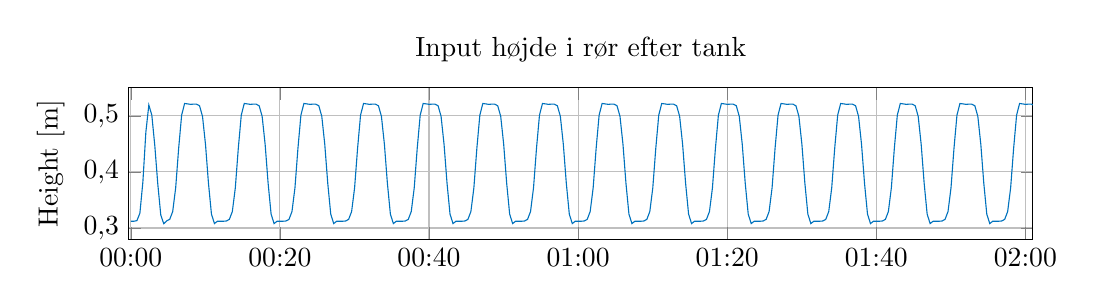
\begin{tikzpicture}

\begin{axis}[%
/pgf/number format/1000 sep={.},/pgf/number format/use comma,
width=4.521in,
height=.7566in,
at={(0.758in,0.481in)},
scale only axis,
xmin=-13.9733315078526,
title={Input højde i rør efter tank },
xmax=6050.45254290018,
xtick={0,1000,2000,3000,4000,5000,6000,7000,8000},
xticklabels={{00:00},{00:20},{00:40},{01:00},{01:20},{01:40},{02:00},{},{}},
%xlabel={Time [hh:mm]},
xmajorgrids,
ymin=0.28,
ymax=0.55,
ylabel={Height [m]},
ymajorgrids,
axis background/.style={fill=white}
]
\addplot [color=mycolor1,solid,forget plot]
  table[row sep=crcr]{%
1	0.312023251728134\\
21	0.312023249248491\\
41	0.313138414051669\\
61	0.326407936305141\\
81	0.381997703162978\\
101	0.470815867610163\\
121	0.519510061802365\\
141	0.501318732196232\\
161	0.446991990334918\\
181	0.378629775152903\\
201	0.323425157927926\\
221	0.307611772797364\\
241	0.312704231743349\\
261	0.315364784289658\\
281	0.329313448452517\\
301	0.371599902771225\\
321	0.442036405727331\\
341	0.501390997061537\\
361	0.522134625957773\\
381	0.521439921581776\\
401	0.520589133516734\\
421	0.520996119305126\\
441	0.520882715260118\\
461	0.518086829318264\\
481	0.499148503119224\\
501	0.449201077704583\\
521	0.379770972259138\\
541	0.324785916393953\\
561	0.307879632744135\\
581	0.312048759866851\\
601	0.31204380765778\\
621	0.31205923660724\\
641	0.312471245607916\\
661	0.315374578361834\\
681	0.329313094015343\\
701	0.371599917605447\\
721	0.44203640471571\\
741	0.501390997170403\\
761	0.522134625943674\\
781	0.52143992158365\\
801	0.520589133516488\\
821	0.520996119305158\\
841	0.520882715260114\\
861	0.518086829318264\\
881	0.499148503119224\\
901	0.449201077704583\\
921	0.379770972259138\\
941	0.324785916393953\\
961	0.307879632744135\\
981	0.312048759866851\\
1001	0.31204380765778\\
1021	0.31205923660724\\
1041	0.312471245607916\\
1061	0.315374578361834\\
1081	0.329313094015343\\
1101	0.371599917605447\\
1121	0.44203640471571\\
1141	0.501390997170403\\
1161	0.522134625943674\\
1181	0.52143992158365\\
1201	0.520589133516488\\
1221	0.520996119305158\\
1241	0.520882715260114\\
1261	0.518086829318264\\
1281	0.499148503119224\\
1301	0.449201077704583\\
1321	0.379770972259138\\
1341	0.324785916393953\\
1361	0.307879632744135\\
1381	0.312048759866851\\
1401	0.31204380765778\\
1421	0.31205923660724\\
1441	0.312471245607916\\
1461	0.315374578361834\\
1481	0.329313094015343\\
1501	0.371599917605447\\
1521	0.44203640471571\\
1541	0.501390997170403\\
1561	0.522134625943674\\
1581	0.52143992158365\\
1601	0.520589133516488\\
1621	0.520996119305158\\
1641	0.520882715260114\\
1661	0.518086829318264\\
1681	0.499148503119224\\
1701	0.449201077704583\\
1721	0.379770972259138\\
1741	0.324785916393953\\
1761	0.307879632744135\\
1781	0.312048759866851\\
1801	0.31204380765778\\
1821	0.31205923660724\\
1841	0.312471245607916\\
1861	0.315374578361834\\
1881	0.329313094015343\\
1901	0.371599917605447\\
1921	0.44203640471571\\
1941	0.501390997170403\\
1961	0.522134625943674\\
1981	0.52143992158365\\
2001	0.520589133516488\\
2021	0.520996119305158\\
2041	0.520882715260114\\
2061	0.518086829318264\\
2081	0.499148503119224\\
2101	0.449201077704583\\
2121	0.379770972259138\\
2141	0.324785916393953\\
2161	0.307879632744135\\
2181	0.312048759866851\\
2201	0.31204380765778\\
2221	0.31205923660724\\
2241	0.312471245607916\\
2261	0.315374578361834\\
2281	0.329313094015343\\
2301	0.371599917605447\\
2321	0.44203640471571\\
2341	0.501390997170403\\
2361	0.522134625943674\\
2381	0.52143992158365\\
2401	0.520589133516488\\
2421	0.520996119305158\\
2441	0.520882715260114\\
2461	0.518086829318264\\
2481	0.499148503119224\\
2501	0.449201077704583\\
2521	0.379770972259138\\
2541	0.324785916393953\\
2561	0.307879632744135\\
2581	0.312048759866851\\
2601	0.31204380765778\\
2621	0.31205923660724\\
2641	0.312471245607916\\
2661	0.315374578361834\\
2681	0.329313094015343\\
2701	0.371599917605447\\
2721	0.44203640471571\\
2741	0.501390997170403\\
2761	0.522134625943674\\
2781	0.52143992158365\\
2801	0.520589133516488\\
2821	0.520996119305158\\
2841	0.520882715260114\\
2861	0.518086829318264\\
2881	0.499148503119224\\
2901	0.449201077704583\\
2921	0.379770972259138\\
2941	0.324785916393953\\
2961	0.307879632744135\\
2981	0.312048759866851\\
3001	0.31204380765778\\
3021	0.31205923660724\\
3041	0.312471245607916\\
3061	0.315374578361834\\
3081	0.329313094015343\\
3101	0.371599917605447\\
3121	0.44203640471571\\
3141	0.501390997170403\\
3161	0.522134625943674\\
3181	0.52143992158365\\
3201	0.520589133516488\\
3221	0.520996119305158\\
3241	0.520882715260114\\
3261	0.518086829318264\\
3281	0.499148503119224\\
3301	0.449201077704583\\
3321	0.379770972259138\\
3341	0.324785916393953\\
3361	0.307879632744135\\
3381	0.312048759866851\\
3401	0.31204380765778\\
3421	0.31205923660724\\
3441	0.312471245607916\\
3461	0.315374578361834\\
3481	0.329313094015343\\
3501	0.371599917605447\\
3521	0.44203640471571\\
3541	0.501390997170403\\
3561	0.522134625943674\\
3581	0.52143992158365\\
3601	0.520589133516488\\
3621	0.520996119305158\\
3641	0.520882715260114\\
3661	0.518086829318264\\
3681	0.499148503119224\\
3701	0.449201077704583\\
3721	0.379770972259138\\
3741	0.324785916393953\\
3761	0.307879632744135\\
3781	0.312048759866851\\
3801	0.31204380765778\\
3821	0.31205923660724\\
3841	0.312471245607916\\
3861	0.315374578361834\\
3881	0.329313094015343\\
3901	0.371599917605447\\
3921	0.44203640471571\\
3941	0.501390997170403\\
3961	0.522134625943674\\
3981	0.52143992158365\\
4001	0.520589133516488\\
4021	0.520996119305158\\
4041	0.520882715260114\\
4061	0.518086829318264\\
4081	0.499148503119224\\
4101	0.449201077704583\\
4121	0.379770972259138\\
4141	0.324785916393953\\
4161	0.307879632744135\\
4181	0.312048759866851\\
4201	0.31204380765778\\
4221	0.31205923660724\\
4241	0.312471245607916\\
4261	0.315374578361834\\
4281	0.329313094015343\\
4301	0.371599917605447\\
4321	0.44203640471571\\
4341	0.501390997170403\\
4361	0.522134625943674\\
4381	0.52143992158365\\
4401	0.520589133516488\\
4421	0.520996119305158\\
4441	0.520882715260114\\
4461	0.518086829318264\\
4481	0.499148503119224\\
4501	0.449201077704583\\
4521	0.379770972259138\\
4541	0.324785916393953\\
4561	0.307879632744135\\
4581	0.312048759866851\\
4601	0.31204380765778\\
4621	0.31205923660724\\
4641	0.312471245607916\\
4661	0.315374578361834\\
4681	0.329313094015343\\
4701	0.371599917605447\\
4721	0.44203640471571\\
4741	0.501390997170403\\
4761	0.522134625943674\\
4781	0.52143992158365\\
4801	0.520589133516488\\
4821	0.520996119305158\\
4841	0.520882715260114\\
4861	0.518086829318264\\
4881	0.499148503119224\\
4901	0.449201077704583\\
4921	0.379770972259138\\
4941	0.324785916393953\\
4961	0.307879632744135\\
4981	0.312048759866851\\
5001	0.31204380765778\\
5021	0.31205923660724\\
5041	0.312471245607916\\
5061	0.315374578361834\\
5081	0.329313094015343\\
5101	0.371599917605447\\
5121	0.44203640471571\\
5141	0.501390997170403\\
5161	0.522134625943674\\
5181	0.52143992158365\\
5201	0.520589133516488\\
5221	0.520996119305158\\
5241	0.520882715260114\\
5261	0.518086829318264\\
5281	0.499148503119224\\
5301	0.449201077704583\\
5321	0.379770972259138\\
5341	0.324785916393953\\
5361	0.307879632744135\\
5381	0.312048759866851\\
5401	0.31204380765778\\
5421	0.31205923660724\\
5441	0.312471245607916\\
5461	0.315374578361834\\
5481	0.329313094015343\\
5501	0.371599917605447\\
5521	0.44203640471571\\
5541	0.501390997170403\\
5561	0.522134625943674\\
5581	0.52143992158365\\
5601	0.520589133516488\\
5621	0.520996119305158\\
5641	0.520882715260114\\
5661	0.518086829318264\\
5681	0.499148503119224\\
5701	0.449201077704583\\
5721	0.379770972259138\\
5741	0.324785916393953\\
5761	0.307879632744135\\
5781	0.312048759866851\\
5801	0.31204380765778\\
5821	0.31205923660724\\
5841	0.312471245607916\\
5861	0.315374578361834\\
5881	0.329313094015343\\
5901	0.371599917605447\\
5921	0.44203640471571\\
5941	0.501390997170403\\
5961	0.522134625943674\\
5981	0.52143992158365\\
6001	0.520589133516488\\
6021	0.520996119305158\\
6041	0.520882715260114\\
6061	0.518086829318264\\
};
\end{axis}
\end{tikzpicture}%
\caption{The output of the last pipe.}
\label{fig:MPC_test_output_second_test_with_constraints}
\end{figure}

It is clear from the figure that the output is not even close to be constant. I fluctuates between two values, the constant input, approximately 0,31 meters, and 0,51 meters. In the top and bottom of the curve, it can be seen that the curve level off. The bottom is due to the tank is empty and therefore, the input, that goes into the tank from the first pipe, goes right into the second pipe without storing any wastewater in the tank. When the top levels off the tank starts to be filled up and as it goes down the tank is emptied. It was discovered that the reason for the top is due to constraints on the upper bound for the input, this however is not a wanted feature. It was desired to get a constant output or a minimum of variations in the output, which is not achieved. Through several tries of changing the parameters of the constraints, e.g. lessen the controller constraint a solution was not found, in every case the output looked similar to the one shown in figure \ref{fig:MPC_test_output_second_test_with_constraints}.







